%% @Author: CHAOUECH OLFA
%  @Date:   2022-06
%% @Class:  PFE de L DSI- Iset Rades, Tunisie.

\documentclass[a4paper, oneside, 12pt, final]{extreport}
\usepackage{graphicx}
\usepackage[table]{xcolor}
\usepackage{colortbl}
\usepackage[first=0,last=9]{lcg}
\newcommand{\ra}{\rand0.\arabic{rand}}	
\usepackage{color, colortbl}
\usepackage{multirow}
\usepackage{numprint}
\usepackage{setspace}
\onehalfspacing
\parindent 0.5cm
\usepackage{makeidx}
\usepackage{fancyhdr}
\usepackage{graphicx}
\usepackage{wrapfig}
\usepackage{tikzducks}
\usepackage{floatflt}
\pagestyle{fancy}
\headsep=50pt
\headheight=50pt
\renewcommand\headrulewidth{1pt}
\fancyhead[C]{}
\fancyhead[L]{\leftmark }
\fancyhead[R]{}
\renewcommand{\footrulewidth}{1pt}
\fancyfoot[C]{\textbf{\thepage}} 
\fancyfoot[L]{Chaouech Olfa}
\fancyfoot[R]{2021-2022}
\makeindex
\definecolor{LightCyan}{rgb}{0.88,1,1}

\usepackage[lined,boxed,commentsnumbered, french, ruled,vlined,linesnumbered]{algorithm2e}
\usepackage{amsthm}
\newtheorem{theorem}{Theorem}[chapter]
\newtheorem{definition}{Definition}[chapter]
\newtheorem{exemple}{Example}[chapter]


%\usepackage[nottoc]{tocbibind}
\addcontentsline{toc}{section}{References}

\providecommand{\keywords}[1]{\textbf{\textit{Mots clés---}} #1}
\providecommand{\keywordss}[1]{\textbf{\textit{Keywords---}} #1}

\usepackage{etoolbox}
%\makeatletter
%\patchcmd{\thebibliography}{%
%  \chapter*{\bibname}\@mkboth{\MakeUppercase\bibname}%{\MakeUppercase\bibname}}{%
%  \section{References}}{}{}
%\makeatother



\usepackage[nottoc]{tocbibind}

\textwidth 16cm
\textheight 25cm
\topmargin -3cm
\oddsidemargin 1cm
\usepackage{hyperref}
% set font encoding for PDFLaTeX or XeLaTeX
\usepackage{ifxetex}
\ifxetex
  \usepackage{fontspec}
\else
  \usepackage[T1]{fontenc}
  \usepackage[utf8]{inputenc}
  \usepackage{lmodern}
\fi


% Enable SageTeX to run SageMath code right inside this LaTeX file.
% documentation: http://mirrors.ctan.org/macros/latex/contrib/sagetex/sagetexpackage.pdf
%\usepackage{sagetex}


\newcommand{\reportTitle} {%
  %\textsc{Graduation Project Report}
  \textsc{ Projet de Fin d'Etudes}
}
\vspace{5pt}
\newcommand{\reportAuthor} {%
  Olfa \textsc{CHAOUECH}%
}
\vspace{5pt}
\newcommand{\reportSubject} {%
 Projet de Fin d'Etudes \\Système de Gestion des formations en ligne%
}

\newcommand{\dateSoutenance} {%
  12/06/2022%
}
\vspace{5pt}
\newcommand{\studyDepartment} {%
  CNUDST %Statistique
}
\vspace{5pt}
\newcommand{\ESSAI} {%
  %Higher School of Statistics and Information Analysis
  Institut Supérieur des
  Études Technologiques de Rades
  Département : Technologies de l’Informatique
  
}
\vspace{5pt}
%\newcommand{\codePFE} {% Reference
%  Code PFE%
%}

\newcommand{\juryPresident} {%
  \textbf{Encadrant entreprise}: \textsc{Mr. CHOKRI BEN ROMDHANE}
}


\newcommand{\juryMemberOne} {%
  \textbf{Encadrant ISET}: \textsc{Mr. Bassem BOUGHZELA}
}


%\newcommand{\Encadrant} {%
  %Mr Bassem \textsc{Boughzala}%
%}
%\newcommand{\juryMemberTwoDesc} {%
 % Reviewer% Examiner, Reporter
%}

%\newcommand{\juryMemberThree} {%
%	M. Ben Foulen \textsc{Fouleni}%
%}
%\newcommand{\juryMemberThreeDesc} {%
%	Supervisor% Examiner, Reporter
%}

%\newcommand{\juryMemberFour} {%
%	M. Ben Foulen \textsc{Fouleni}%
%}
%\newcommand{\juryMemberFourDesc} {%
%	Mentor% Examiner, Reporter
%}


\newcommand{\specialcell}[1]{%
  \begin{tabularx}{\textwidth}{@{}X@{}}#1\end{tabularx}%
}

%%%%%%%%%%%%%%%%%%%%%%%%%%%%%%%%%%%%%%%%%%%%%%%%%%%%%%%
% Add your own commands here
%%%%%%%%%%%%%%%%%%%%%%%%%%%%%%%%%%%%%%%%%%%%%%%%%%%%%%%
\newcommand{\MyCommand} {%
  Does nothing really%
}


% used in maketitle
\title{\reportSubject}
\vspace{5pt}
\author{\reportAuthor}

% Enable SageTeX to run SageMath code right inside this LaTeX file.
% documentation: http://mirrors.ctan.org/macros/latex/contrib/sagetex/sagetexpackage.pdf
%\usepackage{sagetex}

\hypersetup{
  pdftitle={\reportTitle~-~\reportSubject},
  pdfauthor={\reportAuthor},
  pdfsubject={\reportSubject},
  pdfkeywords={report} {internship} {pfe} {enis}
}

\usepackage{graphics}
\usepackage{graphicx}


\usepackage[acronym,toc,section=chapter]{glossaries}
\makeglossaries

\newacronym{abc}{ABC}{A contrived acronym}
\newacronym{efg}{EFG}{Another acronym}
\newacronym{svm}{SVM}{Support Vector Machines}

\pagenumbering{roman} 

\usepackage[utf8]{inputenc}
\usepackage[french]{babel}

\begin{document}
%\thispagestyle{empty}
\begin{titlepage}
\begin{center}


%%%%%%%%%%%%%%%%%%%%%%%%%%%%%%%%%%%%%%%%%%%%%%%
% THE HEADER
%%%%%%%%%%%%%%%%%%%%%%%%%%%%%%%%%%%%%%%%%%%%%%%


\includegraphics[scale=0.25]{embleme.jpg}


{%
  \fontsize{9pt}{9pt}\selectfont%
  \begin{tabular}{c}
    R\'epublique Tunisienne \\
    Minist\`ere de l'Enseignement Supérieur et de la Recherche Scientifique \\%
    \ESSAI{}\\ 
  \end{tabular}
}
\vspace{10pt}




\includegraphics[scale=0.54]{iset.jpg}
\vspace{5pt}

%%%%%%%%%%%%%%%%%%%%%%%%%%%%%%%%%%%%%%%%%%%%%%%
% THE PAGE CONTENT
%%%%%%%%%%%%%%%%%%%%%%%%%%%%%%%%%%%%%%%%%%%%%%%

 {%
  \renewcommand*{\familydefault}{\defaultFont}
  \fontsize{46pt}{46pt}\selectfont%
  % MEMOIRE\\%
  %\reportTitle{}%\\\textsc{Report}\\%
}

\vspace{5pt}


{\textit{Rapport de Projet de Fin d'Etudes}}\\

\vspace{5pt}
{\textbf{\large Licence en Technologies de l'Informatique:  Développement des systèmes d'Information (DSI)}}\\
\vspace{5pt}

\includegraphics[scale=0.4]{logo-essai.png}\\




%\textbf{\textit{Sous la direction de}}\\

 {%
	\fontsize{11pt}{11pt}\selectfont%
	%{\bfseries\Large\sc \Encadrant}\\
}%
 {%
  \renewcommand*{\familydefault}{\defaultFont}
  \fontsize{27pt}{27pt}\selectfont%
  \rule{1\textwidth}{.4pt}\\
  
  \reportSubject{}\\%
 
  \rule{1\textwidth}{.4pt}
}

\vspace{5pt}
%Soutenu le\, \dateSoutenance\,\, %devant le Jury compos\'e de :\\
\textbf{\textit{Réalisé par}}\\
\vspace{5pt}

{%
	\fontsize{11pt}{11pt}\selectfont%
	{\bfseries\Large\sc \reportAuthor}\\
}%
\vspace{5pt}
\textbf{\textit{Encadré par:}}\\
\vspace{5pt}
\juryPresident{}\\

\juryMemberOne{}

%Soutenu le \dateSoutenance, devant la commission d'examen:\\

\begin{tabular}{p{0.3\linewidth} p{0.15\linewidth}}
%  \juryPresident{} & \juryPresidentDesc{}\\
  %\juryMemberOne{} & \juryMemberOneDesc{}\\
 % \juryMemberTwo{} & \juryMemberTwoDesc{}\\
 % \juryMemberThree{} & \juryMemberThreeDesc{}\\
%  \juryMemberFour{} & \juryMemberFourDesc{}\\
\end{tabular}

%\vfill


\textbf{\textit{Projet de Fin d'Etudes fait au}}\\

\studyDepartment\\
\vspace{25pt}
\textbf{Code PFE} : DSI-22-08~~~~~~~~~~~~~~~~~~~~~~~~~~~~~~~~~~~~~
\textbf{Année universitaire} : 2021/2022
%\includegraphics[scale=0.4]{logo-studyDepartment.jpg}
\end{center}
\end{titlepage}

% ###############################
% # HELP COMMANDS               #
% ###############################
%
% -1 \part{part}
%  0 \chapter{chapter}
%  1 \section{section}
%  2 \subsection{subsection}
%  3 \subsubsection{subsubsection}
%  4 \paragraph{paragraph}
%  5 \subparagraph{subparagraph}


%%%%%%%%%%%%%%%%%%%%%%%%%%%%%%%%%%%%%%%%%%%%%%%%%%%%%%%
% Dédicace et Remerciements
%%%%%%%%%%%%%%%%%%%%%%%%%%%%%%%%%%%%%%%%%%%%%%%%%%%%%%%

%\chapter*{Dedication}
\chapter*{D\'edicace}
%\addcontentsline{toc}{chapter}{Dedication}
\thispagestyle{empty}
%
%For all they have endured to satisfy all my needs and wishes

\begin{center}
{\it 
	
A ... pour son(leur) sacrifice et son(leur) soutien, \\
en témoignage de mon infinie reconnaissance et mon profond attachement \\
\vspace{1cm}
A tous ceux qui me sont chers...

}
\end{center}
%
%\nopagebreak{%
% And maybe a quote here
% \raggedright\hspace{5.75cm} To all of you,~\\
%\raggedright\hspace{7.75cm} I dedicate this work.
%  \raggedleft\normalfont\large\itshape{} \reportAuthor\par%
%}
%
%\cleardoublepage%

%\chapter*{Thanks}
\chapter*{Remerciements}
%\addcontentsline{toc}{chapter}{Thanks}
\thispagestyle{empty}
%
%Au terme de ce travail (A l'issue de ce travail), je tiens à remercier M., Mme, Pr., Dr. pour sa disponibilité et ses conseils judicieux. \\
A l'heure où ce travail s'achève, je suis heureuse de pouvoir exprimer ici ma gratitude envers tous ceux qui ont contribué de près ou de loin à son accomplissement.\\
Tout d'abord, je tiens à remercier vivement mon encadrant académique Monsieur Bassem Boughzela qui a accepté de diriger ce travail et l'a enrichi par ses conseils et ses recommandations pertinentes. Je tiens à le remercier vivement pour ses précieux conseils et orientations, son soutien continu et surtout la confiance qu'il m'a accordée.\\
J'ai eu l'honneur d'avoir été dirigée du côté technique par Monsieur Chokri Ben Romdhane. Je lui témoigne toute ma gratitude pour ses encouragements, ses remarques constructives et sa disponibilité.\\
Merci à tout le personnel du  Centre National Universitaire de Documentation Scientifique et
Technique (CNUDST), pour leur accueil, leur soutien et leur gentillesse.\\
Je voudrais aussi exprimer ma gratitude à tous mes enseignants et mes collègues de l'Institut Supérieur des Etudes Technologiques de Rades (ISET Rades).
%Je n'aurais jamais pu réaliser ce projet sans la précieuse aide et sans le soutien d'un grand nombre de personnes dont la générosité, la bonne humeur et l'intérêt manifestés à l'égard de mon PFE m'ont permis de progresser. \\

%En premier lieu, je tiens à remercier mon encadrant universitaire, \juryMemberFour{}, pour la confiance qu'il m'a accordée en acceptant d'encadrer ce travail, pour ses multiples conseils et pour toutes les heures qu'il a consacrées à diriger ce travail. \\ 

%Je souhaiterais exprimer ma gratitude à \juryMemberThree{}, pour m’avoir donné envie de réaliser un mémoire sur ... au sein de \og \studyDepartment \fg. Je le remercie également pour son accueil chaleureux à chaque fois que j'ai sollicité son aide, ainsi que pour ses multiples encouragements. J’ai été extrêmement sensible à ses qualités humaines d'écoute et de compréhension tout au long de ce travail de mémoire. \\

%J'aimerais également dire à \juryPresident{} à quel point je suis honorée pour avoir accepté de présider ce jury de PFE. Je suis infiniment gré à  \juryMemberOne{} de s’être rendu disponible et d’avoir accepté la fonction de rapporteur. De même, je suis particulièrement reconnaissant(e) à (\juryMemberTwo{} de l'intérêt qu'il/elle a manifesté à l'égard de ce projet en s'engageant à être rapporteur. \\

%Ma reconnaissance va à ceux qui ont plus particulièrement assuré le soutien affectif de ce travail : mes enseignants ainsi que mes amis. Mes parents... 


\begin{abstract}

Ce travail s’inscrit dans le cadre du Projet de Fin d'Etudes réalisé au sein de \studyDepartment.\\ 
L’objectif de ce projet consiste à automatiser la gestion des formations organisées par Le Centre National Universitaire de documentation Scientifique et Technique (CNUDST) périodiquement au profit de la communauté scientifique tunisienne. 

% les tests de performance 
\keywords{}
\keywordss{SCRUM, PHP, MySql, Wordpress, Agil, UML} \\

\vspace{1.5cm}
\centerline{\bf Abstract}
\vspace{0.6cm}

The present work is part of a graduation project carried out within the company \studyDepartment.\\ This project aims to automate the management of formation organized by the National University Center for Scientific and Technical Documentation (CNUDST) periodically for the benefit of the Tunisian scientific community.\\

\keywords{}
\keywordss{SCRUM, PHP, MySql, Wordpress, Agil, UML}
\end{abstract}

%%%%%%%%%%%%%%%%%%%%%%%%%%%%%%%%%%%%%%%%%%%%%%%%%%%%%%%
% Divers chapitres
%%%%%%%%%%%%%%%%%%%%%%%%%%%%%%%%%%%%%%%%%%%%%%%%%%%%%%%

\tableofcontents
%\addcontentsline{toc}{chapter}{\contentsname}

\listoffigures
%\addcontentsline{toc}{chapter}{Liste des Figures}
\listoftables
%\addcontentsline{toc}{chapter}{Liste des Tableaux}
%\listofalgorithms
%\addcontentsline{toc}{chapter}{Liste des algorithmes}
\cleardoublepage

\newpage
\pagenumbering{arabic}
\chapter*{Introduction Générale}
\label{chap:general_intorduction}
%% @Author: OLFA CHAOUECH
%  @Date:  09/2022
%% @Class:  PFE de l'ISET Rades.


\markboth{\MakeUppercase{Introduction}}{}%
\addcontentsline{toc}{chapter}{Introduction}%


Les services web ont envahi tous les secteurs d'activité tels que les secteurs du transport, de la santé, de l'économie et notamment le secteur de l'éducation.

Le recours à Internet pour gérer des évènements en ligne, des workshops, des formations, des réunions.., connaît une croissance rapide depuis de nombreuses années et particulièrement après la pandémie de COVID 2019.\\
En Tunisie, la plupart des institutions publiques et privées emploient les services gratuits offerts par les plateformes étrangères telles que "Microsoft Forms" et "Google Forms" pour gérer leurs évènements en ligne.\\
Cependant, l'instance nationale de protection des données personnelles (INPDP) a récemment déclaré que l'usage de ce type de services gratuits se traduit par une fuite des données massive dans le milieu universitaire.
Par conséquent, elle a rappelé dans son article publié le 28 octobre 2021, l'interdiction de recours à ce type de services.\\
Dans ce contexte, le Centre National Universitaire de Documentation Scientifique et Technique (CNUDST), souhaité automatiser la gestion des formations qu'il organise périodiquement au profit de la communauté scientifique tunisienne en développant sa propre application au lieu d'utiliser les services gratuits tel que "Google Forms".
Ce projet d'automatisation a été proposé en tant que PFE.\\
Ainsi, dans le cadre des études de troisième année en licence technologie de l'informatique spécialité "Développement des systèmes d'information (DSI)", nous avons effectué notre stage de Projet de Fin d'Etudes (PFE) au sein du CNUDST.\\
Ce dernier dispose d'un site web déployé moyennant le CMS wordpress qui utilise PHP comme langage de programmation et MySql comme base de données. Les modules de gestion des formations à développer intégreront le site web via le développement d'un nouveau thème pour assurer les inscriptions aux formations en ligne et un plugin pour gérer les formations et leurs inscriptions à ces formations.\\
Le présent rapport décrit la démarche que nous avons appliquée pour réaliser notre projet en utilisant l'approche SCRUM.\\
Notre travail est subdivisé en cinq chapitres comme suit: 
\begin{itemize}
\item Dans le premier chapitre «Cadre Général », nous allons présenter le
cadre du projet. En premier lieu, nous allons décrire l'entreprise d'accueil. En second lieu, nous allons mettre le focus sur l'analyse de l'existant et la solution proposée. Enfin, nous allons terminer par la précision du choix du framework de gestion du projet. 
\item Le second chapitre concerne la phase de planification de projet ou sprint 0. Cette phase comprend la spécification des différents besoins fonctionnels et non fonctionnels et le pilotage du projet avec la méthode SCRUM.\\
Nous allons présenter aussi notre environnement de travail matériel et logiciel ainsi que l'architecture logique et physique de notre système.
\item Les trois autres chapitres constituent le corps de notre rapport, ils seront consacrés au développement des sprints. Chaque chapitre fait l'objet d'un sprint.\\
Chaque sprint est un incrément du produit final qui est potentiellement livrable. 

\end{itemize}





\chapter{Cadre général du projet }%
\label{chap:chapterone}


%%%%%%%%%%%%%%%%%%%%%%%%%%%%
% SECTION                  %
%%%%%%%%%%%%%%%%%%%%%%%%%%%%

\textbf{Introduction} \\
Dans ce chapitre nous allons présenter en premier lieu l'entreprise d'accueil CNUDST, d’une   manière   générale, sa structure organisationnelle, ses missions et son historique.\\ En second lieu nous allons nous focaliser sur l'étude des besoins de l'utilisateur, nous allons détailler les besoins fonctionnels et les exigences non fonctionnelles de l'application.\\ En dernier lieu, nous allons traiter la dernière section qui porte sur l'étude de l'existant.
\section{Présentation de l’entreprise}
Le CNUDST est un centre intégré d’information scientifique et technique. Le CNUDST a pour missions essentielles de :
\begin{itemize}
	\item Fournir l’information et la documentation scientifique et technique notamment aux chercheurs, quel que soit leur domaine d’activité.
	\item Collecter, traiter et diffuser la production et les résultats de la recherche scientifique et du développement technologique entrepris en Tunisie ou portant sur la Tunisie.
	\item Permettre un accès convivial à un fonds documentaire couvrant une partie importante de la recherche scientifique et technologique à l’échelle mondiale.
	\item Pratiquer la veille documentaire.
\end{itemize}
Pour ce faire, des applications sous forme de bases et de banques de données ont été développées dans le but de:
\begin{itemize}
	\item Valoriser les résultats des recherches et contribuer à la promotion de la production scientifique tunisienne en assurant sa visibilité sur le web.
	\item Assurer une veille documentaire permanente sur les ressources documentaires accessibles sur le web à titre gratuit ou à tarif préférentiel (programmes en faveur des pays en développement).
	\item Mettre à la disposition des chercheurs la littérature scientifique mondiale nécessaire à leur activité, par la conclusion de licences avec des éditeurs internationaux en différentes spécialités pour l’accès à des revues en texte intégral et des bases et banques de données.
\end{itemize}
\section{Historique}
Le Centre National Universitaire de Documentation Scientifique et Technique est un établissement public à caractère administratif doté de la personnalité civile et de l’autonomie financière, relevant de la tutelle du Ministère de l’Enseignement Supérieur et de la Recherche Scientifique.
Il a été créé par la loi n° 78-59 du 29/12/1978\footnote{\url{http://cnudst.rnrt.tn/wp-content/uploads/2016/07/78-59-fr.pdf}} portant loi de finances pour la gestion 1979 et notamment son article 33, et géré par décret n° 99-2241 du 11/10/1999. 
\section{Organigramme}
\begin{figure}[!p]
	\centering
{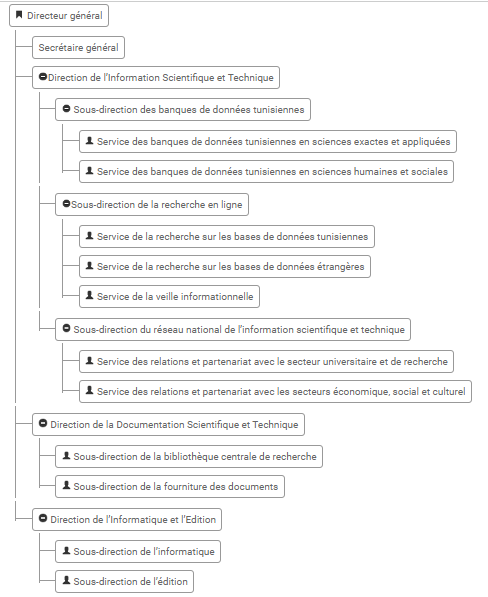
\includegraphics[width=0.95\textwidth]{D) IMAGES/imOrg.png}}
	\caption{Organigramme}
	\label{Org}
\end{figure}

Au sommet, nous trouvons la direction générale. Au deuxième niveau nous trouvons le secrétariat général, la Direction de l'information scientifique et technique, la direction de la documentation scientifique et technique et la direction de l'informatique et de l'édition. Au troisième niveau, nous trouvons les sous-directions.
\newpage
%\section{Problématique}

	

\section{Etude de l’existant } 
Pour gérer les inscriptions aux formations en ligne, le CNUDST lance un formulaire de préinscription via « Google Forms » sur son site web pendant une période bien déterminée.\\
Cependant,  après sa dernière constatation concernant la violation à grande échelle des données personnelles détectée dans le milieu universitaire tunisien, l’instance nationale de protection des données personnelles (INPDP) rappelle dans son article publié le 28 octobre 2021\footnote{\url{https://www.webmanagercenter.com/2021/10/28/474672/violation-a-grande-echelle-des-donnees\\-personnelles-dans-le-milieu-universitaire-tunisien-sinquiete-linpdp}}, l’interdiction du recours aux services gratuits offerts par les plateformes étrangères telles que « Microsoft Forms » et « Google Forms » pour collecter les données personnelles des étudiants, des enseignants et des établissements universitaires.\\Elle invite les responsables à développer des plateformes spécifiques qui seront hébergées sur les sites des établissements concernés.\\Dans ce contexte, notre objectif consiste à développer un plugin et un thème Wordpress pour permettre au CNUDST de gérer les formations qu’il organise et les inscriptions à ces formations au lieu d’utiliser Google Forms.\\
\textbf{Présentation de Google Forms }\\
Google Forms est une application disponible sur la toile qui permet de créer d’une manière très simple et gratuite des fiches personnalisées (fiche d’information, fiche de renseignements, les formulaires d’inscription…).
\begin{figure}[!h]
	\centering
	{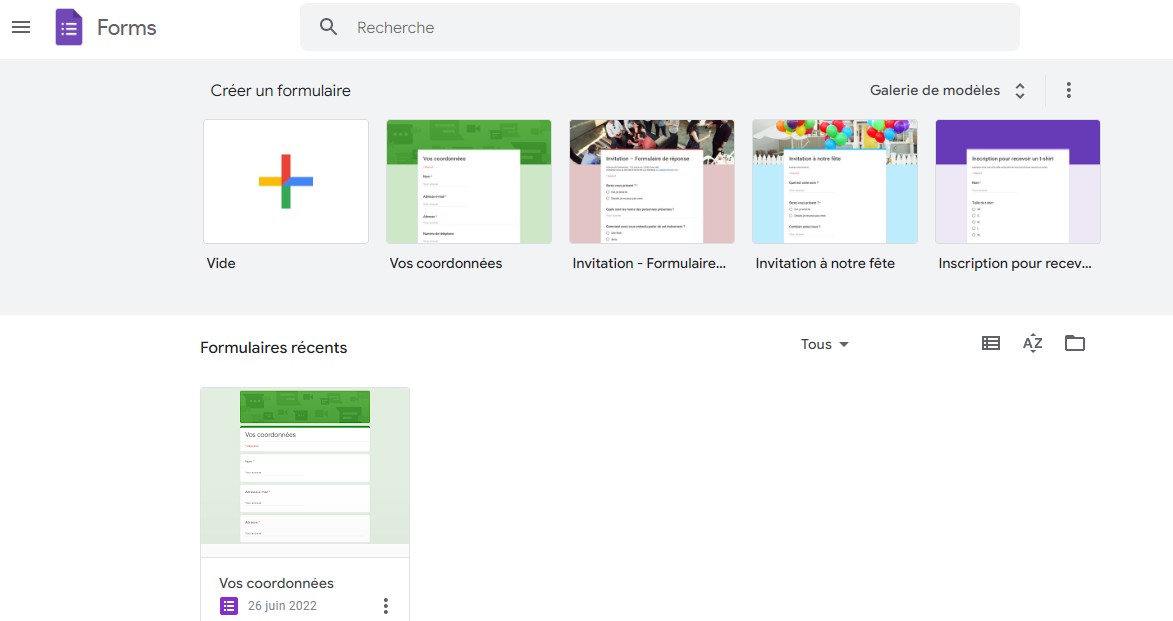
\includegraphics[width=0.95\textwidth]{D) IMAGES/for1.png}}
	\caption{Page d'Accueil Google Forms}
	\label{Org}
\end{figure}
\newpage
L’application présente trois interfaces, la première est une interface qui permet à l’utilisateur de réaliser la conception de sa fiche. \\
\begin{figure}[!h]
	\centering
	{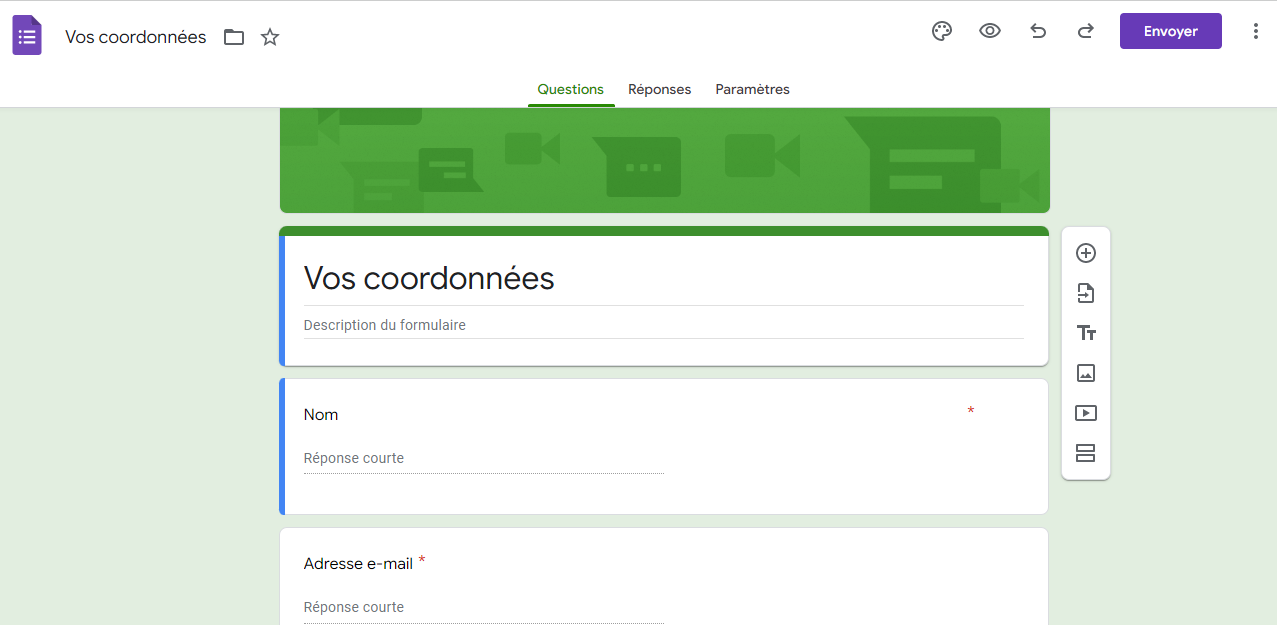
\includegraphics[width=0.95\textwidth]{D) IMAGES/for2.png}}
	\caption{Interface de conception}
	\label{Org}
\end{figure}\\
La deuxième interface est une interface d’aperçu qui permet à l’utilisateur de voir la fiche avant de faire le partage avec les autres via l’envoi du lien vers les E-mails ou bien via les réseaux sociaux (Facebook, Linkdin…).\\
\begin{figure}[!h]
	\centering
	{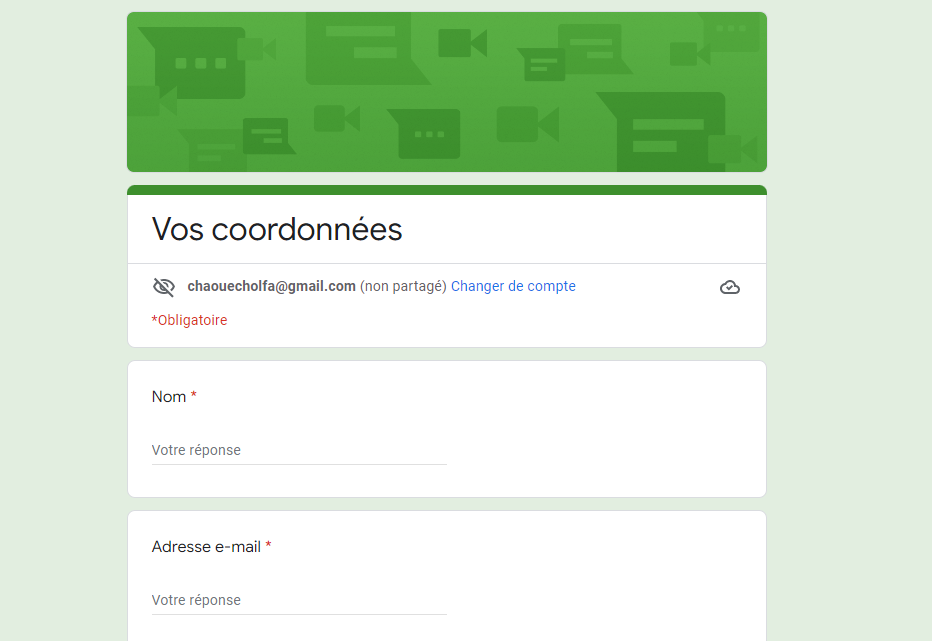
\includegraphics[width=0.95\textwidth]{D) IMAGES/forapp.png}}
	\caption{Interface d'aperçue}
	\label{Org}
\end{figure}
\\
La troisième interface est une interface de réponse qui permet au propriétaire de consulter les réponses. Les informations reçues seront décomposées en base des données.
 Une fois le formulaire d’inscription rempli en ligne, les données seront automatiquement enregistrées dans une feuille de calcul Google sous un format analysable et permettant la tabulation et la représentation graphique de données.
\begin{figure}[!h]
	\centering
	{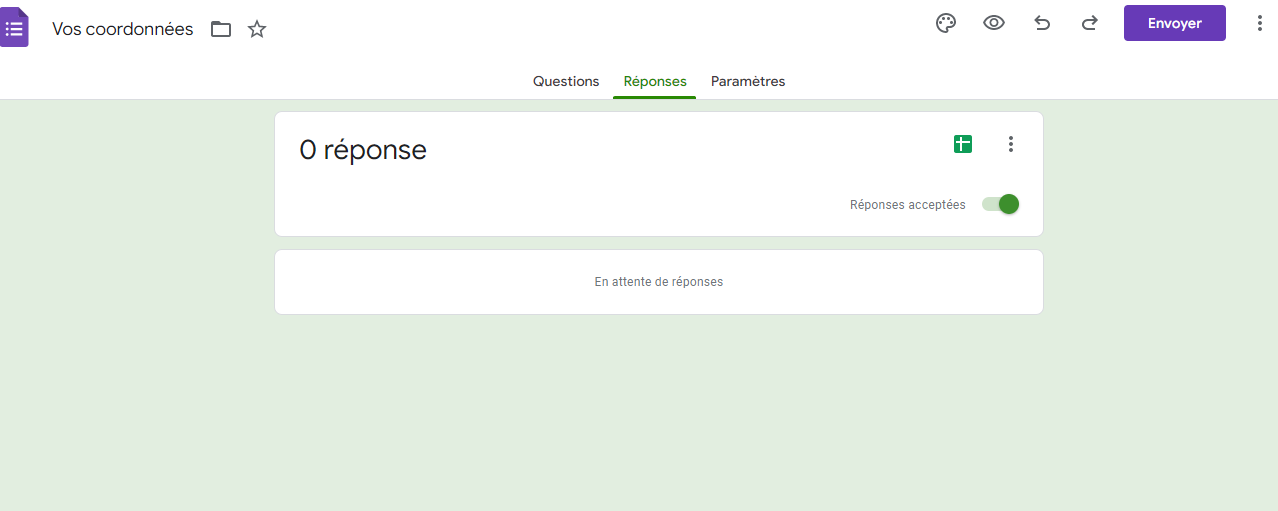
\includegraphics[width=0.95\textwidth]{D) IMAGES/for3.png}}
	\caption{Interface de réponse}
	\label{Org}
\end{figure}
\newpage
\subsection{Critique de l'existant}
Google Forms est un outil de gestion de données basé sur le cloud utilisé pour concevoir et développer des formulaires en ligne, il présente un inconvénient majeur au niveau de sécurité de données personnelles.\\
En effet, selon L’INPDP suite à son usage «Les données personnelles relatives à 13 universités, 203 établissements publics d’enseignement supérieur et 72 établissements privés sont quotidiennement violées, ce qui équivaut à 300 structures d’enseignement et à des milliers d’étudiants, dénonce-t-elle dans un communiqué publié jeudi 28 octobre 2021\footnote{\url{https://www.webmanagercenter.com/2021/10/28/474672/violation-a-grande-echelle-des-donnees\\-personnelles-dans-le-milieu-universitaire-tunisien-sinquiete-linpdp}}. Elle appelle les autorités de tutelle à intervenir pour protéger les données personnelles des étudiants et de tout le personnel travaillant dans le secteur de l’enseignement supérieur.»  
\subsection{Solution proposée}
Le CNUDST dispose d’un site web déployé moyennant le CMS WordPress qui utilise PHP comme langage de programmation et MySQL comme base de données. Les modules de gestion des formations à développer, intégreront le site web via le développement d’un nouveau thème pour assurer les inscriptions aux formations en ligne et un plugin pour gérer les formations et les inscriptions à ces formations.\\
\textbf{Présentation de Wordpress}\\
WordPress est un système de gestion de contenu (SGC) ou CMS (Content Management System) en anglais\footnote{Pour plus d’informations sur le CMS visiter le lien suivant \url{https://www.ionos.fr/digitalguide/hebergement/cms/comparatif-des-meilleurs-cms/} }. Il s’agit d’un système extensible basé sur PHP et MySQL.\\Son architecture est divisée en trois parties principales : les composants de base, les thèmes et les plugins.\\Les composants de base implémentent des fonctionnalités essentielles accessibles via des API que les plugins peuvent utiliser, les thèmes gèrent l'apparence du contenu (par exemple, la mise en page) et les plugins ajoutent des extensions à WordPress.\\
Selon les statistiques fournies par le site \url{https://w3techs.com/}, Wordpress occupe 43.3$\%$ du marché global (de tous les sites web dans le monde) et 65.3 $\%$ concernant le marché des CMS (les sites web créés avec un CMS identifiable). Il est à noter que 33.7 $\%$ des sites web ont été créés sans CMS.
\newpage
\begin{figure}[!h]
	\centering
	{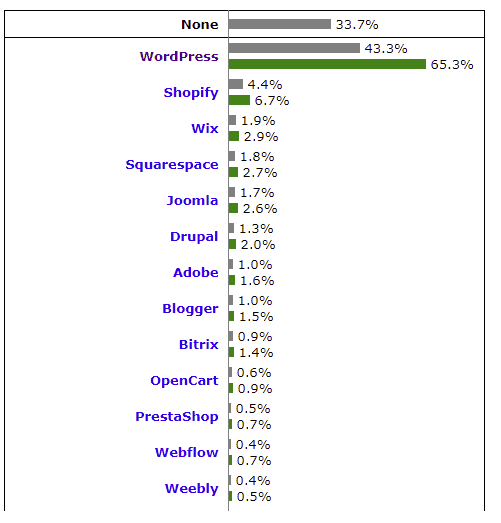
\includegraphics[width=0.75\textwidth]{D) IMAGES/cmsMarche.png}}
	\caption{Part de marché Wordpress}
	\label{CMSWordPress}
\end{figure}

\begin{table}[!h]
	\centering % used for centering table
	\begin{tabular}{ |p{7cm}|p{7cm}| } 
	
		
		\hline% inserts single horizontal line
	\textbf{Avantages} & \textbf{Inconvénients} \\
		\hline
		 Grande Communauté & Les fonctionnalités de CMS nécessitent des extensions supplémentaires\\ 
		 	\hline  
		Faibles coûts d'installation et de configuration & Les plugins ont souvent des failles de sécurité   \\ 
			\hline
		 Interface utilisateur intuitive & Stabilité et performances réduites\\
		  	\hline
		 Intégration facile des plugins & Mises à jour fréquentes de sécurité, ce qui conduit à une administration supplémentaire et parfois lourde  \\ 
	  
		\hline \hline
	
	\end{tabular}
	\begin{flushright}
		\footnotesize Source: Digital guide ionos: Comparatif de CMS 2022 .\end{flushright}
	\caption{Avantages et Inconvénients de WordPress}
\end{table}
Par mesure de sécurité, le CNUDST a choisi de développer ses propres plugins au lieu d'utiliser les plugins fournis par WordPress.\\
Notre objectif consiste donc à développer un plugin pour assurer la gestion des thèmes de formation, des formations et des inscriptions en ligne\footnote{voir la carte mentale du projet à l'annexe 1}.

\section{Choix du framework de gestion de projet}
Au cours des dernières décennies, de nouvelles méthodes sont apparues pour gérer des projets et développer des logiciels. L'idéologie agile était
généralement définie avec le manifeste agile en 2001 et est largement utilisée pour la gestion de projets logiciels. Scrum est
la méthode la plus courante au sein d'agile et est devenue l'un des outils les plus populaires dans le développement de logiciels.\\
Scrum
a une position forte dans le développement de logiciels avec ses rôles définis, son accent sur la collaboration, sa compréhension, sa visibilité, son processus efficace et son développement rapide.

L'objectif de cette section consiste à mettre l'accent sur la façon dont Scrum est appliqué. 
\subsection{Présentation de l’approche agile}
Certains chercheurs ont défini "Agile" comme une philosophie. En effet, selon\\ \cite{highsmith2001agile}"Agile implique d'être efficace et maniable. Un processus Agile est à la fois léger et suffisant. La légèreté est un moyen de rester maniable. \cite{boehm2004balancing} décrit les méthodes Agiles comme "une excroissance d'une expérience de prototypage et de développement rapide ainsi que la résurgence d'une philosophie selon laquelle la programmation est un processus artisanal plutôt qu'industriel"
La suffisance est une question de rester dans le jeu." De sa part, \cite{larman2004agile} a déclaré : « Il n'est pas possible de définir exactement les méthodes agiles, car les pratiques spécifiques varient. Cependant, des itérations limitées dans le temps avec des raffinements adaptatifs et évolutifs des plans et des objectifs".\\
Une autre manière pour décrire les méthodes Agiles consiste à énoncer les pratiques de base partagées par les différentes méthodes Agiles. Selon la définition de \cite{boehm2004balancing} qui est plus basée sur la pratique ",  en général, les méthodes agiles sont des processus très légers qui utilisent des cycles d'itération courts ; Impliquer activement les utilisateurs pour établir, hiérarchiser et vérifier les exigences ; et s'appuyer sur des connaissances tacites au sein d'une équipe plutôt que sur la documentation ".\\
Plus récemment, \cite{abbas2008historical} définit la méthode Agile comme étant "une méthode adaptative, itérative et incrémentale et orientée vers les clients.
\begin{itemize}
	\item Adaptative\\ Une méthode ouverte aux changements dans la technologie et les exigences, de plus elle répond à des retours sur des travaux antérieurs. \cite{fowler2008new} a déclaré qu'un processus adaptatif permet de contrôler l'imprévisibilité.
	\item Itératif et incrémental\\ Le logiciel est développé en plusieurs itérations, chacune de la planification à la livraison.\\
	À chaque itération, une partie du système est développée, testée et améliorée tandis qu'une nouvelle partie est en cours de développement. À chaque itération, la fonctionnalité sera améliorée.\\
	De plus, le système se développe progressivement à mesure que de nouvelles fonctionnalités sont ajoutées à chaque version.
	Après chaque itération(s), une release\footnote{Une release peut être définie comme une période de temps à l’issue de laquelle une version du livrable est proposée. Si une release possède une durée de 30 jours et que les sprints ont une durée de 15 jours, la release comportera alors 2 sprints } sera livrée au client afin d'avoir un retour d'expérience.
	\item Orientée vers les gens\\ 
	Dans une méthode Agile, les personnes sont les principaux moteurs de la réussite du projet.
	Par conséquent, le rôle du processus dans une méthode Agile est d'aider l'équipe de développement à déterminer la meilleure façon de gérer le travail.\\
	De plus, une méthode Agile met l'accent sur la communication en face à face au sein de l'équipe et avec le client qui est étroitement impliqué dans le processus de développement plutôt que sur des documents écrits."\\
	Parmi les méthodes Agiles nous citons eXtreme Programming(XP), SCRUM, Crystal Clear, Feature Driver Developpement(FDD), Lean Software Development, Dynamic System Developpement Methodology(DSDM) et Kanban.\\
	De nouvelles recherches indiquent que 52\% d'organisations utilisent la méthode SCRUM\footnote{\cite{sverrisdottir2014role}}.\\\cite{sverrisdottir2014role}, indique que"dans les méthodes agiles, les mesures de réussite d'un projet ne se limitent pas aux paramètres classiques tels que le temps, le coût et la qualité.\\ La mesure la plus importante est la fonctionnalité du produit, cette mesure est suivie par d'autres facteurs tels que la qualité, le temps/le calendrier et les aspects financiers, la taille des équipes est également importante pour le succès.\\ Il a défini trois catégories pour la taille des équipes, petite, moyenne et grande (plus de 25 personnes).\\
	Il a prouvé que plus les équipes sont petites, plus il est probable que le projet sera réussi.
	\newpage

	\begin{figure}[!h]
		\centering
		{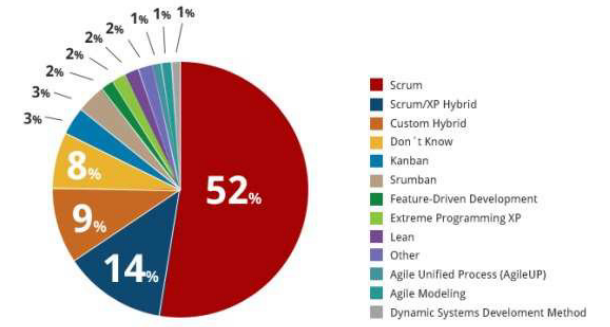
\includegraphics[width=0.85\textwidth]{D) IMAGES/agile.png}}
		\caption{Méthodes Agile}
		\label{Org}
	\end{figure}
	
\end{itemize} 

\subsection{Méthode SCRUM}
SCRUM signifie "mêlée" en français. Cette méthode aurait été définie en 1986 lorsque \cite{takeuchi1986new} ont fait des études sur des méthodes afin de développer de nouveaux produits.\\ Ils ont déclaré que "la flexibilité est l'un des facteurs les plus importants dans le processus de développement, et l'aspect le plus important est que le travail de l'équipe de développement représente une unité vers un objectif commun".\\La méthode est simple et facile à comprendre et à suivre.
Scrum met l'accent sur le contrôle du produit et une partie importante de Scrum consiste à diviser les personnes en équipes et à leur donner les moyens d'effectuer les tâches sur lesquelles elles travaillent.\\
Selon \cite{sverrisdottir2014role}, l'une des caractéristiques de Scrum est qu'une équipe Scrum est autocontrôlée, les gens sont encouragés à proposer de nouvelles idées, cela conduit à la transparence dans la prise de décision et à plus de liberté dans le processus de développement.\\La méthode est suivie d'un examen continu pendant toute la durée du développement, dans le but d'adapter les produits et les procédures de travail à l'environnement en constante évolution \footnote{\cite{sutherland2012scrum}}.\\Les connaissances sont considérées comme fondées sur l'expérience et toutes les décisions sont censées être fondées sur la connaissance.\\
Une équipe Scrum se compose de trois rôles qui sont: le Product Owner(PO), le SCRUM Master(SM) et les membres de l'Equipe.\\ Les processus de la méthode SCRUM sont: le User Story, le Product Backlog, le Sprint, le Sprint Backlog, le Burn Down Chart et le sprint meeting review. \\La méthode Scrum est illustrée graphiquement dans la figure suivante:
\begin{figure}[!h]
	\centering
	{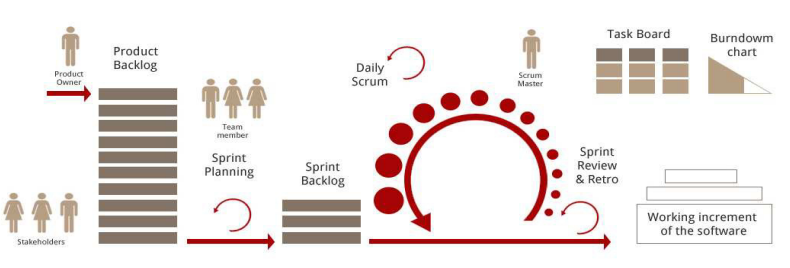
\includegraphics[width=0.95\textwidth]{D) IMAGES/scrum.png}}
	\caption{Cadre de Méthode SCRUM}
	\label{Org}
\end{figure}

\begin{enumerate}
	\item \underline{\textbf{Rôles}}
	
	\begin{itemize}
		\item \textbf{Product Owner} (Directeur du produit)\\
		Le rôle PO est l'un des rôles le plus important dans Scrum et souvent le plus difficile. Il est responsable du financement du projet pendant son cycle de vie et celui qui met le focus sur les exigences et les objectifs du projet. Il définit les spécifications fonctionnelles et établit la liste de priorités. Un PO est une seule personne, pas un groupe de personnes. Il est le représentant de toutes les parties prenantes du projet même le client. La tâche la plus importante du Product Owner est de prendre une décision sur ce qui ne doit pas être priorisé, et
		prendre les conséquences de cette décision. Il est impératif qu'il rejette les nouvelles exigences qui ne sont pas nécessaires, en
		collaboration avec les parties prenantes et l'équipe, au lieu d'ajouter de nouvelles exigences inutiles au Poduct Backlog.
		\item \textbf{SCRUM Master}\\
		La responsabilité de SM est d'assurer que le processus de la méthode SCRUM est appliqué, de plus il supervise la communication au sein de l'équipe et aide l'équipe à se concentrer sur les objectifs du projet.
		\item \textbf{Equipe}\\
		Elle est composée des développeurs, des testeurs, d'architectes et de tout 	autre métier nécessaire à la réalisation de projet.
	\end{itemize}
	\item \underline{\textbf{Processus}}
	
	\begin{itemize}
		\item \textbf{User Story}\\
		Récit utilisateur, il s'agit d'une demande fonctionnelle écrite de façon à mettre en avant les exigences hiérarchisées de l'utilisateur.\\Le product Owner s'engage d'écrire le user story d'une manière précise concernant une seule fonctionnalité. Une fois rédigée, elle va s'ajouter aux autres récits du produit et ensemble forme ce qu'on appelle le "Product backlog".
		\item \textbf{ Le Product Backlog}\\Une sorte de carnet des commandes pour le produit, le product backlog permettre de présenter ce qu'il faut faire pour réaliser les besoins de l'utilisateur et délivrer le User Story. Le Product Backlog va constamment évoluer pour refléter les nouveaux besoins. Une fois d'accord sur le Product Backlog, l'étape suivante consiste à se lancer dans la réalisation de projet ce dernier va se découper en plusieurs itérations nommées sprints dans le jargon de SCRUM.
		\item \textbf{Sprint}\\
		Un Sprint commence par une réunion de planificationn dénommée le \textbf{Sprint planning meeting}, chaque sprint dure de 2 à 4 semaines. Il y aura trois phases pendant le sprint : la phase de développement puis la phase de contrôle et la phase de livraison.\\
		L'ensemble de livraison de Sprints cumulés se nomme le \textbf{Sprint Backlog}.\\
		Durant le sprint il y a des mêlées c'est-à-dire des SCRUM qui vont être organisés chaque jour, ce sont des réunions quotidiennes d'un quart d'heure souvent effectuées au début de la journée. Elles permettent à l'équipe de mesurer l'avancement du projet et de s'assurer de la qualité de délivrable et de respect de délai.\\
		Pendant chaque réunion le SCRUM master tient d'un \textbf{Burn Down chart} pour marquer l'évolution du projet. Chaque membre de l'équipe doit pouvoir exprimer trois choses rapidement:
		\begin{itemize}
			\item Ce que vous avez fait la veille et les problèmes rencontrés.
			\item Ce que vous allez faire aujourd'hui.
			\item Les problèmes qui vous bloquent.
		\end{itemize}  
		L'objectif consiste à identifier et à communiquer les éventuels problèmes sans les résoudre pendant cette séance qui ne dépasse pas les 15 minutes.\\
		A la fin de la réunion, le SRUM Master a mis à jour le Burn Down Chart et déléguer les problèmes identifiés pendant le meeting aux membres de l'équipe.\\
		A la fin de Sprint, c'est-à-dire en général après deux semaines un autre meeting sera organisé, \textbf{le sprint meeting review}, au cours dequel la solution sera présentée au client sous forme de démonstration et d'avoir son retour, des éventuelles améliorations sont suggérées et les problèmes rencontrés seront ajoutés au Product Backlog et priorisés ensuite dans des Sprints. 
		
		
	\end{itemize}
	
\end{enumerate}


\textbf{Conclusion}\\
Tout au long de ce chapitre, nous avons présenté, en premier lieu, l'entreprise d'accueil. En second lieu, nous avons identifié l'existant tout en montrant sa critique et nous avons envisagé par la suite la solution proposée. Enfin, nous avons mis le focus sur la méthodologie utilisée.  

%\chapter{Méthodologies utilisées}%
%\label{chap:2}
%
\textbf{Introduction}\\
Dans ce chapitre nous allons préparer notre planification de projet ou «sprint 0». Cette phase représente une phase importante dans le cycle de développement SCRUM puisqu’elle a une influence directe sur la
réussite des sprints et en particulier le premier.
Nous allons spécifier en premier lieu les différents besoins fonctionnels et non fonctionnels, après nous allons fournir les éléments nécessaires afin de piloter le projet avec la méthode SCRUM. Enfin, nous allons présenter notre environnement de travail matériel et logiciel et l'architecture logique et physique de notre système.   
\section{Spécification des besoins}
Cette partie sert à identifier les fonctionnalités attendues dans l’application. Elle résume les besoins fonctionnels auxquels doit répondre l’application.

\subsection{Les besoins fonctionnels}
Le Centre National Universitaire de documentation Scientifique et Technique (CNUDST)
souhaite automatiser la gestion des formations qu’il organise périodiquement au profit de
la communauté scientifique tunisienne.\\
On peut distinguer trois types de formations qui sont:
\begin{enumerate}
	\item Les ateliers
	\item Les workshops avec éditeurs : sont assurés par les éditeurs de revues, ouvrages ou bases de données scientifiques
	\item Les journées d’information sur les ressources électroniques
\end{enumerate}

Les ateliers: assurés par le personnel du CNUDST portent sur 3 thèmes bien
déterminés à savoir :
\begin{enumerate}
	\item Méthodologie de la recherche bibliographique,
	\item Utilisation des outils de référencement bibliographique : cas de Endnote,
	\item Utilisation des outils bibliographiques et bibliométriques.
	Ces ateliers subdivisent en deux catégories : 
	
\end{enumerate}
Ces ateliers peuvent être publics et gratuits, animés dans les locaux du CNUDST en général au mois de Janvier ou des ateliers ciblés, payants et sur demande des
institutions.\\
La participation aux ateliers gratuits dans les locaux du CNUDST se fait à travers
une préinscription réalisée en ligne. Le processus d’inscription à
ces ateliers se déroule selon les étapes suivantes :
\\
\underline{\textit{Etape1 : Préinscription :}}\\
Un formulaire de préinscription est publié par le CNUDST sur son site
web, pendant une période bien déterminée.\\
L’annonce et l’ouverture des préinscriptions se font en même temps et englobent au
départ toutes les sessions des thèmes.\\
La fermeture de la préinscription se fait sur demande du formateur concerné et
par session, selon le nombre de demandes d’inscription reçues et le nombre de
places disponibles pour chaque session.\\
Le lien devient inaccessible dès que toutes les sessions seront comblées.\\ 
\underline{\textit{Etape 2 : Sélection des préinscriptions :}}\\
La sélection des préinscriptions se fait en se basant sur des critères fixés par
chaque formateur, parmi ces critères :
\begin{itemize}
	\item Le nombre de places (limité).
	\item La qualité de la personne préinscrite (par exemple un chercheur a la
	priorité par rapport à un étudiant, un bibliothécaire ne peut pas assister à
	ce genre d'ateliers, …).
	\item Une seule préinscription par session et par thème est retenue (les
	préinscriptions redondantes, pour le même thème sur des sessions
	différentes, seront rejetées).
\end{itemize}
\underline{\textit{Etape 3 : Demande de confirmation des inscriptions :}}\\
Une demande de confirmation de l’inscription est envoyée à la liste des personnes
sélectionnées pour assister à la formation.\\
Cette liste contient un nombre
supérieur à celui des places disponibles (en moyenne, 10 places) pour combler les
éventuelles absences d’un ou plusieurs participants).\\
\underline{\textit{Etape 4 : Approbation des inscriptions :}}\\
Une liste finale des inscrits est fixée et un e-mail de confirmation des inscriptions
est envoyé aux personnes concernées avec les détails suivants :
\begin{itemize}
	\item Date, heure et lieu de formation
	\item Outils de travail
\end{itemize}
Un atelier payant est organisé à la suite d’une demande issue de la part d’une institution
universitaire ou de recherche ou un établissement privé.\\
Le lieu de la formation et les outils matériels et techniques nécessaires pour le bon
déroulement de la formation sont à la charge du demandeur de la formation.\\ Ces ateliers
portent sur les mêmes thèmes que les ateliers gratuits.\\
Le processus de déroulement de ce type de formation est le suivant :\\
\underline{\textit{Etape1: Réception d’une demande de formation}}\\
Le CNUDST reçoit une correspondance, au nom du directeur général,
ayant pour objet une demande de formation.\\
\underline{\textit{Etape2: Traitement de la demande:}}\\
La demande sera remise au responsable de l’organisation des formations pour la
traiter:
\begin{itemize}
	\item Si la correspondance ne contient pas les informations nécessaires, le responsable
	de l’organisation des formations envoie une nouvelle correspondance, à travers la
	direction générale, dans
	laquelle il sera demandé de fournir plus d’informations sur la demande tout en
	mentionnant : les thèmes de formations, les tarifs, le nombre maximum de
	personnes qui peuvent assister (avec une copie de l’arrêté du 13 Février 2017
	fixant les tarifs des services payants rendus par le CNUDST). 
	\item Si la correspondance contient les informations nécessaires, le responsable de
	l’organisation des formations commence le traitement de la demande en
	collaboration avec l’équipe des formateurs (disponibilité des dates et des
	formateurs).
\end{itemize}
\underline{\textit{Etape2: Traitement de la demande:}}\\
Une correspondance est envoyée au demandeur de la formation en vue de confirmation de
la demande de formation et de transmission de participants (Nom
et Prénom) pour préparer les attestations. Cette correspondance contient les
informations suivantes :
\begin{itemize}
	\item Le ou les thèmes de formation.
	\item Les dates de formations.
	\item La liste des formateurs.
	\item Le programme des formations.
\end{itemize}
\underline{\textit{Etape 4 : Confirmation de la formation}}\\	
Réception d’une confirmation envoyée par le représentant du
demandeur de la formation.


\subsection{Les besoins non fonctionnels}
Les besoins non fonctionnels caractérisent le système et affectent le flux réel de l'application. Ce sont des besoins techniques qui décrivent la plupart des contraintes auxquelles le système est soumis et qui permet d'assurer sa mise en oeuvre et son bon fonctionnement.
Dans ce cas notre projet doit respecter un ensemble de besoins pour avoir une meilleure performance telles que:
\begin{itemize}
	\item \textbf{La Fiabilité :}\\
	Cette exigence veut dire que notre application doit effectuer les fonctionnalités prévues dans les
	conditions normales d’utilisations. C’est-à-dire dans le cas où il n'y a aucune exception, notre application
	doit accomplir sa mission.
	\item \textbf{La Portabilité :}\\
	Notre application doit être compatible avec n’importe quel système d’exploitation.
	\item \textbf{L'Ergonomie:}\\
	Les interfaces de notre solution doivent être ergonomiques et conviviales, elles doivent être aussi  lisible et facile à manipuler par n'importe quel utilisateur sans difficultés.
	\item \textbf{L'Extensibilité :}\\
    Notre application doit adopter une implémentation claire et simple et un code lisible pour permettre en cas de
	besoin, une modification facile des fonctionnalités existantes ainsi que l’ajout des nouvelles
	fonctions.
	\item \textbf{La Performance:}\\Au niveau du temps de réponse, nous allons veiller, aussi, à ce que notre site ait un temps de
	réponse rapide pour garantir la fluidité de navigation et une expérience utilisateur de qualité. Nous
	proposons d’évaluer la performance (rapidité) avec le service en ligne PageSpeed :
	https://pagespeed.web.dev/
	\item \textbf{La Compatibilité}\\
	Notre site web est développé avec les technologies récentes et il est compatible avec la plupart
	des navigateurs du marché :
	\begin{itemize}
		\item Navigateurs desktop: Google Chrome, Mozilla Firefox, Microsoft Edge, Opera, Safari. 
		\item Navigateurs mobile: Chrome, Firefox, Opera, Samsung Internet, UC Browser, Brave Browser…
		
	\end{itemize}
	
	Nous allons tester la compatibilité de note application avec le navigateur le plus populaire
	avec le service en ligne BowserLing sur le site : \\https://www.browserling.com/
	\item \textbf{La Sécurité:}\\
	La sécurité générale de notre site est assurée par un backup automatisé pour
	sauvegarder les données. Le développement de notre site est effectué tout en respectant
	le guide de test de sécurité Web OWASP.\\
	Notre site garantit la sécurité des données personnelles :
	\begin{itemize}
		\item Exigences à respecter au niveau du remplissage du formulaire,
		\item Validation de tous les champs,
		\item Gestion des droits d’accès,
		\item Protection contre les spam et les abus avec le service reCAPTCHA de Google,
	\end{itemize}
\end{itemize}
\section{Modélisation des besoins}
Les diagrammes de notre application sont effectués grâce à l'outil de conception graphique \textbf{draw.io}.
Il est disponible en ligne sur le lien suivant:\url{https://www.diagram.net}.\\
Le diagramme de cas d'utilisation de notre système est représenté comme suit:
%\newpage
\begin{figure}[!h]
	\centering
	{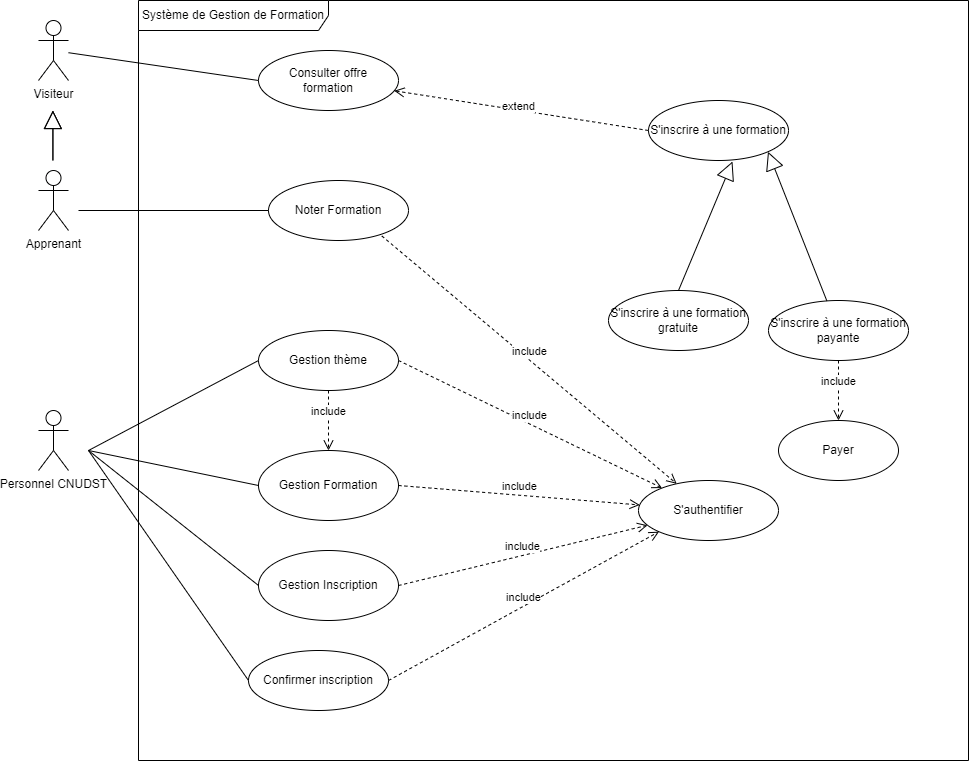
\includegraphics[width=1\textwidth]{D) IMAGES/casutlglobal.png}}
	\caption{Diagramme des cas d'utilisation globale du système}
	\label{Diagramme3}
\end{figure}

\section{Pilotage du projet avec SCRUM}
\subsection{Rôles de SCRUM}
\begin{table}[!h]
	\centering % used for centering table
	\begin{tabular}{ |c|c| } 
		
		
		\hline% inserts single horizontal line
		\centering{\textbf{~~~~Rôle SCRUM~~~~}} & \textbf{~~~~Personnes Affectées~~~~} \\
		\hline
		Product Owner & Chokri Ben Romdhane\\ 
		\hline  
		SCRUM Master & Bassem Boughzala   \\ 
		\hline
		Developpers Team & Olfa Chaouech  \\
		\hline
		
		
		
	\end{tabular}
	
	\caption{équipe et rôles Scrum}
\end{table}
\section{Backlog du produit}
Le tableau ci-dessous présente le « Backlog » du produit initial. Le « Backlog » se traduit par un
ensemble de «user stories» qui décrivent les fonctionnalités attendues de l’application.\\
A chaque «user story» est associé un identifiant et une priorité.\\
Une ou plusieurs user stories peuvent être regroupées dans un EPIC.
\begin{table}[!h]
	\centering % used for centering table
	\begin{tabular}{|p{4cm}|p{1cm}|p{8.5cm}|c|}
		\hline
		\textbf{EPIC}&\textbf{Id} & \centering{\textbf{User Story}} & \textbf{Priorité}\tabularnewline
		\hline
		& US1  & En tant qu'administrateur, je peux créer un thème &1\\
		\cline{2-4}
		& US2  & En tant qu'utilisateur, je peux consulter la liste des thèmes (All Events) &2\\
		\cline{2-4}
		\multirow{-2}{2cm}{Gestion thème de formation}& US3&En tant qu'administrateur, je peux mettre à jour un thème de formation & 3\\
		\cline{2-4}
		& US4  & En tant qu'utilisateur, je peux consulter les détails d'un thème&4\\
		\cline{2-4}
		\hline
		
		& US5  & En tant qu'administrateur, je peux intégrer des formations dans le thème&5\\
		\cline{2-4}
		\multirow{-2}{2cm}{Gestion formation}& US6&En tant qu'administrateur, je peux mettre à jour une  formation & 6\\
		\hline
		& US7  & En tant qu'utilisateur je peux consulter la liste des
		formations&7\\
		\cline{2-4}
		& US8&En tant qu'utilisateur je peux consulter les détails des
		formations& 8\\
		\cline{2-4}
		\multirow{-3}{3cm}{Consultation des offres de formation}& US9  & 
		En tant qu'utilisateur je veux contacter les responsables du site
		pour avoir plus d’informations sur une offre&9\\
		\hline
		
	& US10&En tant qu'utlisateur je veux m’inscrire pour pouvoir participer à une formation & 10\\
		\cline{2-4}
			\multirow{-2}{4cm}{Inscription à une Formation en ligne}& US11&En tant qu'administrateur ou apprenant, je veux m'authentifier & 11\\
			\cline{2-4}
	& US12&En tant qu'administrateur, je peux confirmer une inscription& 12\\
	
		
			
		\hline
	& US13&En tant qu'apprenant, je veux donner mon avis concernant une formation & 13\\
	\cline{2-4}
	\multirow{-2}{4cm}{Interaction sur le site}& US14&En tant qu'administrateur ou apprenant, je peux modifier une note concernant une formation  & 14\\
	\cline{2-4}
	& US15&En tant qu'administrateur ou apprenant, je peux Supprimer une note concernant une formation  & 15\\
	\hline	
		
	\end{tabular}
	\caption{Tableau : Backlog product}
\end{table}

\section{La planification de release}
La planification de release fournit des informations sur le contenu des sprints, dans le cas de notre
projet, la réalisation de l’application nécessite une release qui commence le $02/05/2022$ et se termine le $02/09/2022$.
\subsection{Durée des sprints}
Après l’estimation de nos « user stories », nous avons partagé notre release sur trois sprints d’une
durée de quatre semaines.
\subsection{Planning des sprints}
Voici la répartition temporelle des trois sprints que nous allons réaliser dans les chapitres suivants.
\begin{figure}[!h]
	\centering
	{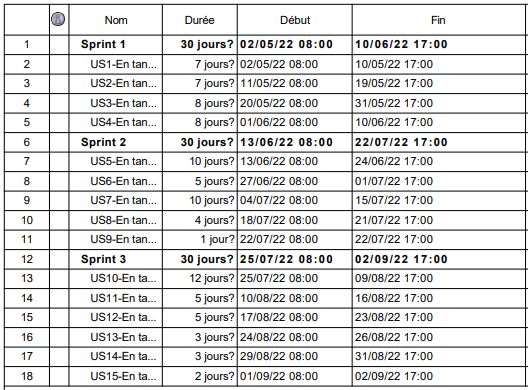
\includegraphics[width=0.95\textwidth]{D) IMAGES/PlanningdesSprints.png}}
	\caption{Planning des sprints-feuille de calcul (ProjectLibre)}
	\label{Org}
\end{figure}
\begin{figure}[!h]
	\centering
	{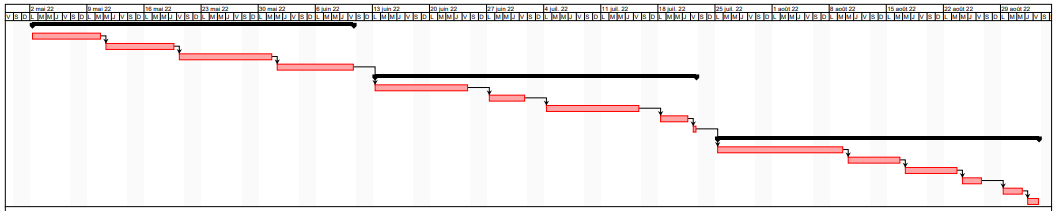
\includegraphics[width=0.95\textwidth]{D) IMAGES/PlanningDesSprintsGantt.png}}
	\caption{Planning des sprints-diagramme de Gantt (ProjectLibre)}
	\label{Org}
\end{figure}
\section{Environnement de travail}
\subsection{Environnement matériel}
Nous présentons les caractéristiques de nos outils matériels utilisés pour la réalisation de notre application.
\begin{table}[!h]
	\centering % used for centering table
	\begin{tabular}{ |c|p{10cm}| } 
		
		
		\hline% inserts single horizontal line
		\centering{\textbf{Type}} & \textbf{~~~~~~Désignation} \\
		\hline
	Marque & ASUS\\ 
		\hline  
		Processeur & Intel(R) Core(TM):7-106567 CPU@1.30 GHZ 1.50 GHZ   \\ 
		\hline
		RAM & 20 GO  \\
		\hline
	Système d'exploitation & Windows 10 \\ 
		
		\hline 
		Architecture & 64 bit \\
		\hline
		
	\end{tabular}
	\begin{flushright}
		\footnotesize Source: Digital guide ionos: Comparatif de CMS 2022 .\end{flushright}
	\caption{Caractéristiques de l'Environnement Matériel}
\end{table}
\subsection{Environnement logiciel}
\begin{enumerate}
	\item Outils de développement et modélisation
	\begin{itemize}
		\item Pour le développement, nous avons utilisé : \textbf{VSCode} et\textbf{WAMP}.
		\item Pour la modélisation, nous avons utilisé: \textbf{draw.io}
	\end{itemize}
	\item Langage de programmation et framework\\
	Les langages et framework de programmation que nous avons utilisés.
	\begin{itemize}
		\item \textbf{Côté front-end}
		\begin{itemize}
			\item HTML, CSS et JavaScript.
		\end{itemize}
		\item \textbf{Côté back-end}
		\begin{itemize}
			\item Langage php,
			\item Rest API,
			\item MySQL , 
		\end{itemize}
    	\item \textbf{Logiciel de gestion de projet Scrum}\\
    	Pour la gestion du projet par la méthode SCRUM, nous avons utilisé: Trello et Project Libre.
		\item \textbf{Côté hébergement et déploiement}
		\begin{itemize}
			\item Github.git
			\item Latex
		\end{itemize}
		
	\end{itemize}
\end{enumerate}
\subsection{Présentation des logiciels et outils utilisés}
	
	\begin{itemize}
		\item  \begin{minipage}{.10\textwidth}%
			
\includegraphics[width=0.95\textwidth]{D) IMAGES/html.png}
		\end{minipage}%
		L’HyperText Mark up Langage, généralement abrégé HTML, est le langage de balisage conçu pour représenter les pages web.
C’est un langage permettant d’écrire de l’hypertexte, d’où son nom. HTML permet également de structurer sémantiquement et logiquement et de mettre en forme le contenu des pages, d’inclure des ressources multimédias dont des images, des formulaires de saisie et des éléments 
programmables tels que des applets. 
	\item \begin{minipage}{.10\textwidth}%
		
\includegraphics[width=0.95\textwidth]{D) IMAGES/css.png}
	\end{minipage}%	
Les feuilles de style en cascade, généralement appelées CSS de l'anglais Cascading Style Sheets, forment un langage informatique qui décrit la présentation des documents HTML et XML. Les standards définissant CSS sont publiés par le World Wide Web Consortium (W3C). Introduit au milieu des années 1990, CSS devient couramment utilisé dans la conception de sites web et bien pris en charge par les navigateurs web dans les années 2000 (Wikipédia,2019a et IWM,2020).
 \item \begin{minipage}{.15\textwidth}%
 	
\includegraphics[width=0.95\textwidth]{D) IMAGES/latex.jpg}
 \end{minipage}% 
\LaTeX est un langage informatique, un logiciel libre et un système de composition de document.\\
Ce système a été développé par le chercheur américain "Leslie Lamport". Il s'agit d'une version simplifiée du système Tex de "Donald Knuth".\\
Nous avons choisi \LaTeX  car il permet de rédiger des documents dont la mise en page est réalisée automatiquement en se conformant du mieux possible à des normes typographiques.\\
Le tableau suivant permet de comparer  \LaTeX~et Word.  

\begin{table}[ht]
	\centering
	\begin{tabular}{c|cc}
		\hline
		& Word, OpenOffice & \LaTeX   \\
		\hline
		\rowcolor{LightCyan}
		Apprentissage à court terme& Facile & Dur  \\
		Changement de la mise en page& Facile & Dur\\
		\rowcolor{LightCyan}
		Interaction avec le document& Direct & Indirect \\
		Fonctionnalités avancées& Includes & Par morceaux \\
		\rowcolor{LightCyan}
		Multi-plateforme& Non & Oui  \\
		Formules mathématiques& Récent & Très robuste  \\
		\rowcolor{LightCyan}
		Longévité de la compatibilité& Courte & Longue  \\
		Algorithme de mise en page& Pauvre & Evolué\\
		\rowcolor{LightCyan}
		Structuration du document & Optionnelle & Obligatoire \\
		Nombre de polices& Très élevé & Par morceaux \\
		\rowcolor{LightCyan}
		Bibliographie& Externe & Automatique  \\
		Edition avec ChemDraw & Directe & Indirecte  \\
		\rowcolor{LightCyan}
		Images inclues dans le fichier & Oui & Non \\
		Poids d'un fichier & $\approx$ 10 Mo & $\approx$ 500 Ko\\
		\hline
		
	\end{tabular}
	\caption{Comparaison Word /\LaTeX}
\end{table}


     
 	\item  \begin{minipage}{.10\textwidth}%
 		
\includegraphics[width=0.95\textwidth]{D) IMAGES/java.png}
 	\end{minipage}% 
 JavaScript : JavaScript est un langage de programmation de scripts principalement employé dans les pages web interactives mais aussi pour les serveurs avec l'utilisation, par exemple, de Node.js. C'est un langage orienté objet à prototype, c'est-à-dire que les bases du langage et ses principales interfaces sont fournies par des objets qui ne sont pas des instances de classes, mais qui sont chacun équipés de constructeurs permettant de créer leurs propriétés, et notamment une propriété de prototypage qui permet d'en créer des objets héritiers personnalisés.
 \item  \begin{minipage}{.15\textwidth}%
 	
\includegraphics[width=0.95\textwidth]{D) IMAGES/php.jpg}
 \end{minipage}% 
PHP: Hypertext Preprocessor, plus connu sous son sigle PHP (sigle auto-référentiel), est un langage de programmation libre, principalement utilisé pour produire des pages Web dynamiques via un serveur HTTP, mais pouvant également fonctionner comme n'importe quel langage interprété de façon locale. PHP est un langage impératif orienté objet.

PHP a permis de créer un grand nombre de sites web célèbres, comme Facebook et Wikipédia. Il est considéré comme une des bases de la création de sites web dits dynamiques mais également des applications web.(Wikipédia)\\
Le, CMS WordPress que nous avons utilisé pour le développement de notre interface web, est écrit avec le langage de script PHP.\\





\item  \begin{minipage}{.15\textwidth}%
	
\includegraphics[width=0.95\textwidth]{D) IMAGES/VSCode.png}
\end{minipage}% 
Visual Studio Code : est un éditeur de code open-source, gratuit et multi-plateforme (Windows, Mac et Linux), développé par Microsoft.
Visual Studio Code prend immédiatement en charge presque tous les principaux langages de programmation et de balisage. Plusieurs d'entre eux sont inclus par défaut, par exemple JavaScript, TypeScript, CSS et HTML, mais d'autres extensions de langage peuvent être trouvées et téléchargées gratuitement à partir de VS Code Marketplace.
\item \begin{minipage}{.25\textwidth}%
	
\includegraphics[width=0.95\textwidth]{D) IMAGES/draw.png}
\end{minipage}%
Pour la modélisation, nous avons utilisé "draw.io" connu aussi sous diagrams.net, il s'agit d'un outil de création de diagrammes gratuit et collaboratif.\\
Il permet aux utilisateurs de créer et de partager des diagrammes dans un navigateur web. 

 \item  \begin{minipage}{.25\textwidth}%
 	
\includegraphics[width=0.95\textwidth]{D) IMAGES/sql.png}
 \end{minipage}% 
C’est un logiciel de gestion et d’administration de base de données. Via une interface graphique 
intuitive, il permet de manipuler (créer, modifier supprimer) des objets, des données, des comptes 
utilisateurs, et d’effectuer toutes les opérations inhérentes à la gestion d’une base de données. Pour 
cela il doit être connecté à un serveur MySQL.
	
\end{itemize}
\section{Architecture de l'application}

\subsection{Architecture physique}
Nous allons choisir une architecture 3-tiers pour notre application. L’architecture à trois
couches est une architecture client-serveur adaptée aux applications web et permet :
\begin{itemize}
	\item Une plus grande flexibilité /souplesse,
	\item Une plus grande sécurité (la sécurité peut être définie pour chaque service),
	\item De meilleures performances (les tâches sont partagées).
\end{itemize}
\begin{figure}[!h]
	\centering
	{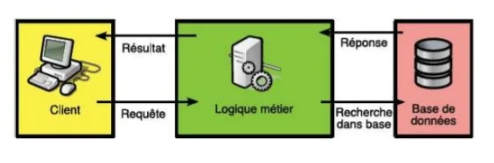
\includegraphics[width=0.85\textwidth]{D) IMAGES/arch.png}}
	\caption{Architecture physique 3-tiers}
	\label{Diagramme3}
\end{figure}
\subsection{Architecture logique}
La démarche MVC est un patron de conception qui sépare les données (le modèle), l’interface 
homme-machine (la vue) et la logique de contrôle(le contrôle).

\begin{figure}[!h]
	\centering
	{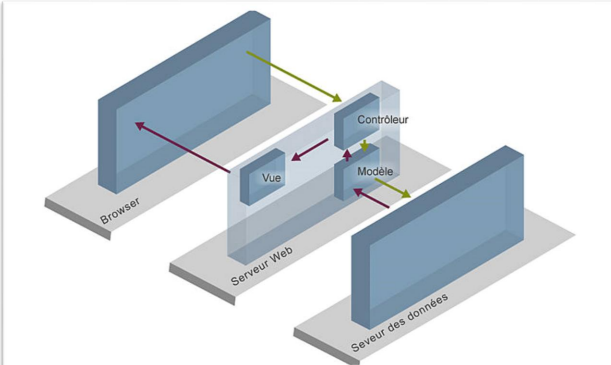
\includegraphics[width=0.65\textwidth]{D) IMAGES/MVC.png}}
	\caption{Architecture logique MVC}
	\label{Diagramme3}
\end{figure}

\begin{itemize}
	\item \textbf{Modèle} : Encapsule le cœur fonctionnel de l’application, le domaine logique.
	\item \textbf{Vue}:Les données sont envoyées par le modèle, à la vue qui les visualise à l’utilisateur.
	\item \textbf{Contrôleur}: Cet objet - car il s'agit aussi d'un objet - permet de faire le lien entre la vue et 
	le modèle lorsqu'une action utilisateur est intervenue sur la vue. C'est cet objet qui aura pour 
	rôle de contrôler les données.
	

\end{itemize}

\textbf{Conclusion}\\
A travers ce chapitre, nous avons spécifié les besoins fonctionnels et non fonctionnels de la solution en premier lieu. En second lieu, nous avons construit notre backlog du produit qui va nous permettre de bien entamer le premier sprint de notre projet que nous allons aborder dans le chapitre suivant.



\chapter{Planification du projet}%
\label{chap:2}

\textbf{Introduction}\\
Dans ce chapitre nous allons préparer notre planification de projet ou «sprint 0». Cette phase représente une phase importante dans le cycle de développement SCRUM puisqu’elle a une influence directe sur la
réussite des sprints et en particulier le premier.
Nous allons spécifier en premier lieu les différents besoins fonctionnels et non fonctionnels, après nous allons fournir les éléments nécessaires afin de piloter le projet avec la méthode SCRUM. Enfin, nous allons présenter notre environnement de travail matériel et logiciel et l'architecture logique et physique de notre système.   
\section{Spécification des besoins}
Cette partie sert à identifier les fonctionnalités attendues dans l’application. Elle résume les besoins fonctionnels auxquels doit répondre l’application.

\subsection{Les besoins fonctionnels}
Le Centre National Universitaire de documentation Scientifique et Technique (CNUDST)
souhaite automatiser la gestion des formations qu’il organise périodiquement au profit de
la communauté scientifique tunisienne.\\
On peut distinguer trois types de formations qui sont:
\begin{enumerate}
	\item Les ateliers
	\item Les workshops avec éditeurs : sont assurés par les éditeurs de revues, ouvrages ou bases de données scientifiques
	\item Les journées d’information sur les ressources électroniques
\end{enumerate}

Les ateliers: assurés par le personnel du CNUDST portent sur 3 thèmes bien
déterminés à savoir :
\begin{enumerate}
	\item Méthodologie de la recherche bibliographique,
	\item Utilisation des outils de référencement bibliographique : cas de Endnote,
	\item Utilisation des outils bibliographiques et bibliométriques.
	Ces ateliers subdivisent en deux catégories : 
	
\end{enumerate}
Ces ateliers peuvent être publics et gratuits, animés dans les locaux du CNUDST en général au mois de Janvier ou des ateliers ciblés, payants et sur demande des
institutions.\\
La participation aux ateliers gratuits dans les locaux du CNUDST se fait à travers
une préinscription réalisée en ligne. Le processus d’inscription à
ces ateliers se déroule selon les étapes suivantes :
\\
\underline{\textit{Etape1 : Préinscription :}}\\
Un formulaire de préinscription est publié par le CNUDST sur son site
web, pendant une période bien déterminée.\\
L’annonce et l’ouverture des préinscriptions se font en même temps et englobent au
départ toutes les sessions des thèmes.\\
La fermeture de la préinscription se fait sur demande du formateur concerné et
par session, selon le nombre de demandes d’inscription reçues et le nombre de
places disponibles pour chaque session.\\
Le lien devient inaccessible dès que toutes les sessions seront comblées.\\ 
\underline{\textit{Etape 2 : Sélection des préinscriptions :}}\\
La sélection des préinscriptions se fait en se basant sur des critères fixés par
chaque formateur, parmi ces critères :
\begin{itemize}
	\item Le nombre de places (limité).
	\item La qualité de la personne préinscrite (par exemple un chercheur a la
	priorité par rapport à un étudiant, un bibliothécaire ne peut pas assister à
	ce genre d'ateliers, …).
	\item Une seule préinscription par session et par thème est retenue (les
	préinscriptions redondantes, pour le même thème sur des sessions
	différentes, seront rejetées).
\end{itemize}
\underline{\textit{Etape 3 : Demande de confirmation des inscriptions :}}\\
Une demande de confirmation de l’inscription est envoyée à la liste des personnes
sélectionnées pour assister à la formation.\\
Cette liste contient un nombre
supérieur à celui des places disponibles (en moyenne, 10 places) pour combler les
éventuelles absences d’un ou plusieurs participants).\\
\underline{\textit{Etape 4 : Approbation des inscriptions :}}\\
Une liste finale des inscrits est fixée et un e-mail de confirmation des inscriptions
est envoyé aux personnes concernées avec les détails suivants :
\begin{itemize}
	\item Date, heure et lieu de formation
	\item Outils de travail
\end{itemize}
Un atelier payant est organisé à la suite d’une demande issue de la part d’une institution
universitaire ou de recherche ou un établissement privé.\\
Le lieu de la formation et les outils matériels et techniques nécessaires pour le bon
déroulement de la formation sont à la charge du demandeur de la formation.\\ Ces ateliers
portent sur les mêmes thèmes que les ateliers gratuits.\\
Le processus de déroulement de ce type de formation est le suivant :\\
\underline{\textit{Etape1: Réception d’une demande de formation}}\\
Le CNUDST reçoit une correspondance, au nom du directeur général,
ayant pour objet une demande de formation.\\
\underline{\textit{Etape2: Traitement de la demande:}}\\
La demande sera remise au responsable de l’organisation des formations pour la
traiter:
\begin{itemize}
	\item Si la correspondance ne contient pas les informations nécessaires, le responsable
	de l’organisation des formations envoie une nouvelle correspondance, à travers la
	direction générale, dans
	laquelle il sera demandé de fournir plus d’informations sur la demande tout en
	mentionnant : les thèmes de formations, les tarifs, le nombre maximum de
	personnes qui peuvent assister (avec une copie de l’arrêté du 13 Février 2017
	fixant les tarifs des services payants rendus par le CNUDST). 
	\item Si la correspondance contient les informations nécessaires, le responsable de
	l’organisation des formations commence le traitement de la demande en
	collaboration avec l’équipe des formateurs (disponibilité des dates et des
	formateurs).
\end{itemize}
\underline{\textit{Etape2: Traitement de la demande:}}\\
Une correspondance est envoyée au demandeur de la formation en vue de confirmation de
la demande de formation et de transmission de participants (Nom
et Prénom) pour préparer les attestations. Cette correspondance contient les
informations suivantes :
\begin{itemize}
	\item Le ou les thèmes de formation.
	\item Les dates de formations.
	\item La liste des formateurs.
	\item Le programme des formations.
\end{itemize}
\underline{\textit{Etape 4 : Confirmation de la formation}}\\	
Réception d’une confirmation envoyée par le représentant du
demandeur de la formation.


\subsection{Les besoins non fonctionnels}
Les besoins non fonctionnels caractérisent le système et affectent le flux réel de l'application. Ce sont des besoins techniques qui décrivent la plupart des contraintes auxquelles le système est soumis et qui permet d'assurer sa mise en oeuvre et son bon fonctionnement.
Dans ce cas notre projet doit respecter un ensemble de besoins pour avoir une meilleure performance telles que:
\begin{itemize}
	\item \textbf{La Fiabilité :}\\
	Cette exigence veut dire que notre application doit effectuer les fonctionnalités prévues dans les
	conditions normales d’utilisations. C’est-à-dire dans le cas où il n'y a aucune exception, notre application
	doit accomplir sa mission.
	\item \textbf{La Portabilité :}\\
	Notre application doit être compatible avec n’importe quel système d’exploitation.
	\item \textbf{L'Ergonomie:}\\
	Les interfaces de notre solution doivent être ergonomiques et conviviales, elles doivent être aussi  lisible et facile à manipuler par n'importe quel utilisateur sans difficultés.
	\item \textbf{L'Extensibilité :}\\
    Notre application doit adopter une implémentation claire et simple et un code lisible pour permettre en cas de
	besoin, une modification facile des fonctionnalités existantes ainsi que l’ajout des nouvelles
	fonctions.
	\item \textbf{La Performance:}\\Au niveau du temps de réponse, nous allons veiller, aussi, à ce que notre site ait un temps de
	réponse rapide pour garantir la fluidité de navigation et une expérience utilisateur de qualité. Nous
	proposons d’évaluer la performance (rapidité) avec le service en ligne PageSpeed :
	https://pagespeed.web.dev/
	\item \textbf{La Compatibilité}\\
	Notre site web est développé avec les technologies récentes et il est compatible avec la plupart
	des navigateurs du marché :
	\begin{itemize}
		\item Navigateurs desktop: Google Chrome, Mozilla Firefox, Microsoft Edge, Opera, Safari. 
		\item Navigateurs mobile: Chrome, Firefox, Opera, Samsung Internet, UC Browser, Brave Browser…
		
	\end{itemize}
	
	Nous allons tester la compatibilité de note application avec le navigateur le plus populaire
	avec le service en ligne BowserLing sur le site : \\https://www.browserling.com/
	\item \textbf{La Sécurité:}\\
	La sécurité générale de notre site est assurée par un backup automatisé pour
	sauvegarder les données. Le développement de notre site est effectué tout en respectant
	le guide de test de sécurité Web OWASP.\\
	Notre site garantit la sécurité des données personnelles :
	\begin{itemize}
		\item Exigences à respecter au niveau du remplissage du formulaire,
		\item Validation de tous les champs,
		\item Gestion des droits d’accès,
		\item Protection contre les spam et les abus avec le service reCAPTCHA de Google,
	\end{itemize}
\end{itemize}
\section{Modélisation des besoins}
Les diagrammes de notre application sont effectués grâce à l'outil de conception graphique \textbf{draw.io}.
Il est disponible en ligne sur le lien suivant:\url{https://www.diagram.net}.\\
Le diagramme de cas d'utilisation de notre système est représenté comme suit:
%\newpage
\begin{figure}[!h]
	\centering
	{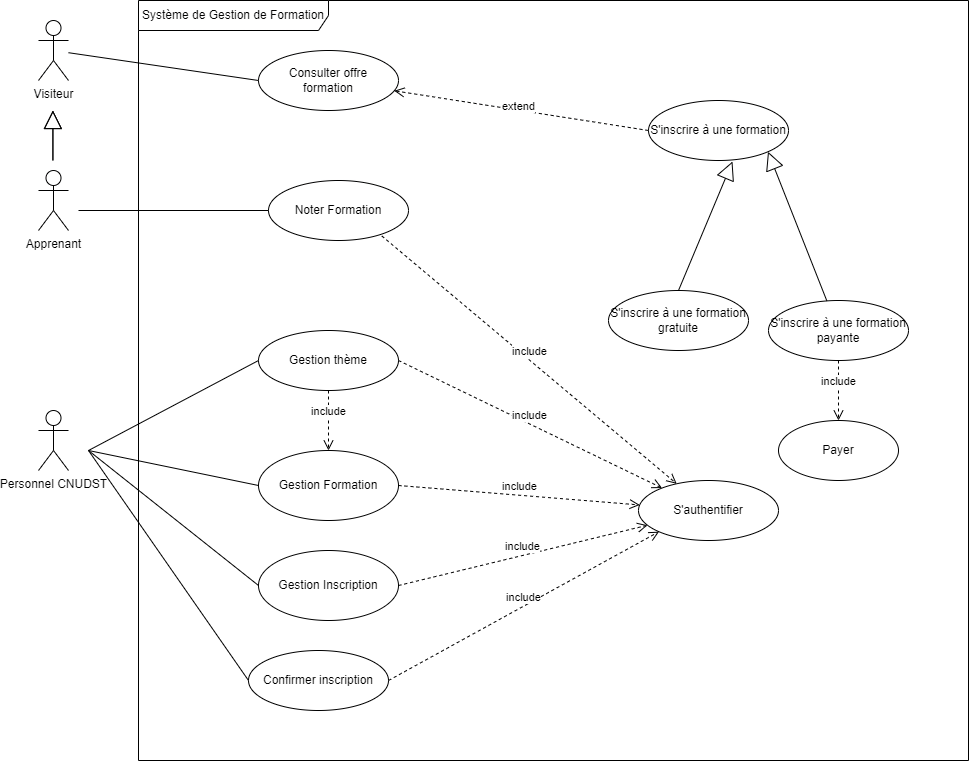
\includegraphics[width=1\textwidth]{D) IMAGES/casutlglobal.png}}
	\caption{Diagramme des cas d'utilisation globale du système}
	\label{Diagramme3}
\end{figure}

\section{Pilotage du projet avec SCRUM}
\subsection{Rôles de SCRUM}
\begin{table}[!h]
	\centering % used for centering table
	\begin{tabular}{ |c|c| } 
		
		
		\hline% inserts single horizontal line
		\centering{\textbf{~~~~Rôle SCRUM~~~~}} & \textbf{~~~~Personnes Affectées~~~~} \\
		\hline
		Product Owner & Chokri Ben Romdhane\\ 
		\hline  
		SCRUM Master & Bassem Boughzala   \\ 
		\hline
		Developpers Team & Olfa Chaouech  \\
		\hline
		
		
		
	\end{tabular}
	
	\caption{équipe et rôles Scrum}
\end{table}
\section{Backlog du produit}
Le tableau ci-dessous présente le « Backlog » du produit initial. Le « Backlog » se traduit par un
ensemble de «user stories» qui décrivent les fonctionnalités attendues de l’application.\\
A chaque «user story» est associé un identifiant et une priorité.\\
Une ou plusieurs user stories peuvent être regroupées dans un EPIC.
\begin{table}[!h]
	\centering % used for centering table
	\begin{tabular}{|p{4cm}|p{1cm}|p{8.5cm}|c|}
		\hline
		\textbf{EPIC}&\textbf{Id} & \centering{\textbf{User Story}} & \textbf{Priorité}\tabularnewline
		\hline
		& US1  & En tant qu'administrateur, je peux créer un thème &1\\
		\cline{2-4}
		& US2  & En tant qu'utilisateur, je peux consulter la liste des thèmes (All Events) &2\\
		\cline{2-4}
		\multirow{-2}{2cm}{Gestion thème de formation}& US3&En tant qu'administrateur, je peux mettre à jour un thème de formation & 3\\
		\cline{2-4}
		& US4  & En tant qu'utilisateur, je peux consulter les détails d'un thème&4\\
		\cline{2-4}
		\hline
		
		& US5  & En tant qu'administrateur, je peux intégrer des formations dans le thème&5\\
		\cline{2-4}
		\multirow{-2}{2cm}{Gestion formation}& US6&En tant qu'administrateur, je peux mettre à jour une  formation & 6\\
		\hline
		& US7  & En tant qu'utilisateur je peux consulter la liste des
		formations&7\\
		\cline{2-4}
		& US8&En tant qu'utilisateur je peux consulter les détails des
		formations& 8\\
		\cline{2-4}
		\multirow{-3}{3cm}{Consultation des offres de formation}& US9  & 
		En tant qu'utilisateur je veux contacter les responsables du site
		pour avoir plus d’informations sur une offre&9\\
		\hline
		
	& US10&En tant qu'utlisateur je veux m’inscrire pour pouvoir participer à une formation & 10\\
		\cline{2-4}
			\multirow{-2}{4cm}{Inscription à une Formation en ligne}& US11&En tant qu'administrateur ou apprenant, je veux m'authentifier & 11\\
			\cline{2-4}
	& US12&En tant qu'administrateur, je peux confirmer une inscription& 12\\
	
		
			
		\hline
	& US13&En tant qu'apprenant, je veux donner mon avis concernant une formation & 13\\
	\cline{2-4}
	\multirow{-2}{4cm}{Interaction sur le site}& US14&En tant qu'administrateur ou apprenant, je peux modifier une note concernant une formation  & 14\\
	\cline{2-4}
	& US15&En tant qu'administrateur ou apprenant, je peux Supprimer une note concernant une formation  & 15\\
	\hline	
		
	\end{tabular}
	\caption{Tableau : Backlog product}
\end{table}

\section{La planification de release}
La planification de release fournit des informations sur le contenu des sprints, dans le cas de notre
projet, la réalisation de l’application nécessite une release qui commence le $02/05/2022$ et se termine le $02/09/2022$.
\subsection{Durée des sprints}
Après l’estimation de nos « user stories », nous avons partagé notre release sur trois sprints d’une
durée de quatre semaines.
\subsection{Planning des sprints}
Voici la répartition temporelle des trois sprints que nous allons réaliser dans les chapitres suivants.
\begin{figure}[!h]
	\centering
	{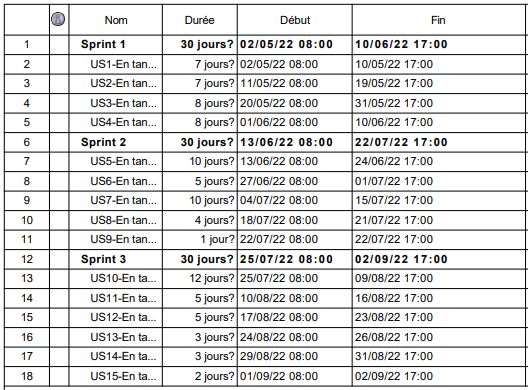
\includegraphics[width=0.95\textwidth]{D) IMAGES/PlanningdesSprints.png}}
	\caption{Planning des sprints-feuille de calcul (ProjectLibre)}
	\label{Org}
\end{figure}
\begin{figure}[!h]
	\centering
	{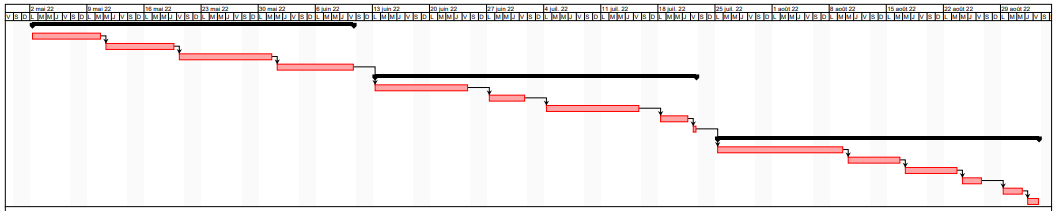
\includegraphics[width=0.95\textwidth]{D) IMAGES/PlanningDesSprintsGantt.png}}
	\caption{Planning des sprints-diagramme de Gantt (ProjectLibre)}
	\label{Org}
\end{figure}
\section{Environnement de travail}
\subsection{Environnement matériel}
Nous présentons les caractéristiques de nos outils matériels utilisés pour la réalisation de notre application.
\begin{table}[!h]
	\centering % used for centering table
	\begin{tabular}{ |c|p{10cm}| } 
		
		
		\hline% inserts single horizontal line
		\centering{\textbf{Type}} & \textbf{~~~~~~Désignation} \\
		\hline
	Marque & ASUS\\ 
		\hline  
		Processeur & Intel(R) Core(TM):7-106567 CPU@1.30 GHZ 1.50 GHZ   \\ 
		\hline
		RAM & 20 GO  \\
		\hline
	Système d'exploitation & Windows 10 \\ 
		
		\hline 
		Architecture & 64 bit \\
		\hline
		
	\end{tabular}
	\begin{flushright}
		\footnotesize Source: Digital guide ionos: Comparatif de CMS 2022 .\end{flushright}
	\caption{Caractéristiques de l'Environnement Matériel}
\end{table}
\subsection{Environnement logiciel}
\begin{enumerate}
	\item Outils de développement et modélisation
	\begin{itemize}
		\item Pour le développement, nous avons utilisé : \textbf{VSCode} et\textbf{WAMP}.
		\item Pour la modélisation, nous avons utilisé: \textbf{draw.io}
	\end{itemize}
	\item Langage de programmation et framework\\
	Les langages et framework de programmation que nous avons utilisés.
	\begin{itemize}
		\item \textbf{Côté front-end}
		\begin{itemize}
			\item HTML, CSS et JavaScript.
		\end{itemize}
		\item \textbf{Côté back-end}
		\begin{itemize}
			\item Langage php,
			\item Rest API,
			\item MySQL , 
		\end{itemize}
    	\item \textbf{Logiciel de gestion de projet Scrum}\\
    	Pour la gestion du projet par la méthode SCRUM, nous avons utilisé: Trello et Project Libre.
		\item \textbf{Côté hébergement et déploiement}
		\begin{itemize}
			\item Github.git
			\item Latex
		\end{itemize}
		
	\end{itemize}
\end{enumerate}
\subsection{Présentation des logiciels et outils utilisés}
	
	\begin{itemize}
		\item  \begin{minipage}{.10\textwidth}%
			
\includegraphics[width=0.95\textwidth]{D) IMAGES/html.png}
		\end{minipage}%
		L’HyperText Mark up Langage, généralement abrégé HTML, est le langage de balisage conçu pour représenter les pages web.
C’est un langage permettant d’écrire de l’hypertexte, d’où son nom. HTML permet également de structurer sémantiquement et logiquement et de mettre en forme le contenu des pages, d’inclure des ressources multimédias dont des images, des formulaires de saisie et des éléments 
programmables tels que des applets. 
	\item \begin{minipage}{.10\textwidth}%
		
\includegraphics[width=0.95\textwidth]{D) IMAGES/css.png}
	\end{minipage}%	
Les feuilles de style en cascade, généralement appelées CSS de l'anglais Cascading Style Sheets, forment un langage informatique qui décrit la présentation des documents HTML et XML. Les standards définissant CSS sont publiés par le World Wide Web Consortium (W3C). Introduit au milieu des années 1990, CSS devient couramment utilisé dans la conception de sites web et bien pris en charge par les navigateurs web dans les années 2000 (Wikipédia,2019a et IWM,2020).
 \item \begin{minipage}{.15\textwidth}%
 	
\includegraphics[width=0.95\textwidth]{D) IMAGES/latex.jpg}
 \end{minipage}% 
\LaTeX est un langage informatique, un logiciel libre et un système de composition de document.\\
Ce système a été développé par le chercheur américain "Leslie Lamport". Il s'agit d'une version simplifiée du système Tex de "Donald Knuth".\\
Nous avons choisi \LaTeX  car il permet de rédiger des documents dont la mise en page est réalisée automatiquement en se conformant du mieux possible à des normes typographiques.\\
Le tableau suivant permet de comparer  \LaTeX~et Word.  

\begin{table}[ht]
	\centering
	\begin{tabular}{c|cc}
		\hline
		& Word, OpenOffice & \LaTeX   \\
		\hline
		\rowcolor{LightCyan}
		Apprentissage à court terme& Facile & Dur  \\
		Changement de la mise en page& Facile & Dur\\
		\rowcolor{LightCyan}
		Interaction avec le document& Direct & Indirect \\
		Fonctionnalités avancées& Includes & Par morceaux \\
		\rowcolor{LightCyan}
		Multi-plateforme& Non & Oui  \\
		Formules mathématiques& Récent & Très robuste  \\
		\rowcolor{LightCyan}
		Longévité de la compatibilité& Courte & Longue  \\
		Algorithme de mise en page& Pauvre & Evolué\\
		\rowcolor{LightCyan}
		Structuration du document & Optionnelle & Obligatoire \\
		Nombre de polices& Très élevé & Par morceaux \\
		\rowcolor{LightCyan}
		Bibliographie& Externe & Automatique  \\
		Edition avec ChemDraw & Directe & Indirecte  \\
		\rowcolor{LightCyan}
		Images inclues dans le fichier & Oui & Non \\
		Poids d'un fichier & $\approx$ 10 Mo & $\approx$ 500 Ko\\
		\hline
		
	\end{tabular}
	\caption{Comparaison Word /\LaTeX}
\end{table}


     
 	\item  \begin{minipage}{.10\textwidth}%
 		
\includegraphics[width=0.95\textwidth]{D) IMAGES/java.png}
 	\end{minipage}% 
 JavaScript : JavaScript est un langage de programmation de scripts principalement employé dans les pages web interactives mais aussi pour les serveurs avec l'utilisation, par exemple, de Node.js. C'est un langage orienté objet à prototype, c'est-à-dire que les bases du langage et ses principales interfaces sont fournies par des objets qui ne sont pas des instances de classes, mais qui sont chacun équipés de constructeurs permettant de créer leurs propriétés, et notamment une propriété de prototypage qui permet d'en créer des objets héritiers personnalisés.
 \item  \begin{minipage}{.15\textwidth}%
 	
\includegraphics[width=0.95\textwidth]{D) IMAGES/php.jpg}
 \end{minipage}% 
PHP: Hypertext Preprocessor, plus connu sous son sigle PHP (sigle auto-référentiel), est un langage de programmation libre, principalement utilisé pour produire des pages Web dynamiques via un serveur HTTP, mais pouvant également fonctionner comme n'importe quel langage interprété de façon locale. PHP est un langage impératif orienté objet.

PHP a permis de créer un grand nombre de sites web célèbres, comme Facebook et Wikipédia. Il est considéré comme une des bases de la création de sites web dits dynamiques mais également des applications web.(Wikipédia)\\
Le, CMS WordPress que nous avons utilisé pour le développement de notre interface web, est écrit avec le langage de script PHP.\\





\item  \begin{minipage}{.15\textwidth}%
	
\includegraphics[width=0.95\textwidth]{D) IMAGES/VSCode.png}
\end{minipage}% 
Visual Studio Code : est un éditeur de code open-source, gratuit et multi-plateforme (Windows, Mac et Linux), développé par Microsoft.
Visual Studio Code prend immédiatement en charge presque tous les principaux langages de programmation et de balisage. Plusieurs d'entre eux sont inclus par défaut, par exemple JavaScript, TypeScript, CSS et HTML, mais d'autres extensions de langage peuvent être trouvées et téléchargées gratuitement à partir de VS Code Marketplace.
\item \begin{minipage}{.25\textwidth}%
	
\includegraphics[width=0.95\textwidth]{D) IMAGES/draw.png}
\end{minipage}%
Pour la modélisation, nous avons utilisé "draw.io" connu aussi sous diagrams.net, il s'agit d'un outil de création de diagrammes gratuit et collaboratif.\\
Il permet aux utilisateurs de créer et de partager des diagrammes dans un navigateur web. 

 \item  \begin{minipage}{.25\textwidth}%
 	
\includegraphics[width=0.95\textwidth]{D) IMAGES/sql.png}
 \end{minipage}% 
C’est un logiciel de gestion et d’administration de base de données. Via une interface graphique 
intuitive, il permet de manipuler (créer, modifier supprimer) des objets, des données, des comptes 
utilisateurs, et d’effectuer toutes les opérations inhérentes à la gestion d’une base de données. Pour 
cela il doit être connecté à un serveur MySQL.
	
\end{itemize}
\section{Architecture de l'application}

\subsection{Architecture physique}
Nous allons choisir une architecture 3-tiers pour notre application. L’architecture à trois
couches est une architecture client-serveur adaptée aux applications web et permet :
\begin{itemize}
	\item Une plus grande flexibilité /souplesse,
	\item Une plus grande sécurité (la sécurité peut être définie pour chaque service),
	\item De meilleures performances (les tâches sont partagées).
\end{itemize}
\begin{figure}[!h]
	\centering
	{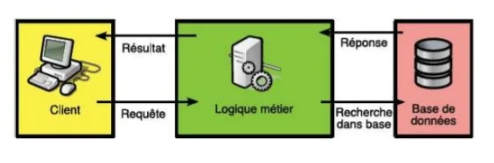
\includegraphics[width=0.85\textwidth]{D) IMAGES/arch.png}}
	\caption{Architecture physique 3-tiers}
	\label{Diagramme3}
\end{figure}
\subsection{Architecture logique}
La démarche MVC est un patron de conception qui sépare les données (le modèle), l’interface 
homme-machine (la vue) et la logique de contrôle(le contrôle).

\begin{figure}[!h]
	\centering
	{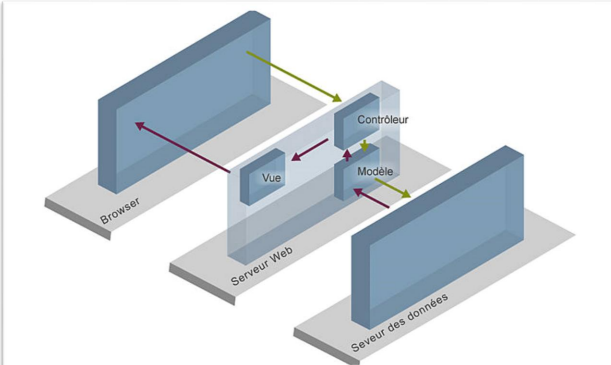
\includegraphics[width=0.65\textwidth]{D) IMAGES/MVC.png}}
	\caption{Architecture logique MVC}
	\label{Diagramme3}
\end{figure}

\begin{itemize}
	\item \textbf{Modèle} : Encapsule le cœur fonctionnel de l’application, le domaine logique.
	\item \textbf{Vue}:Les données sont envoyées par le modèle, à la vue qui les visualise à l’utilisateur.
	\item \textbf{Contrôleur}: Cet objet - car il s'agit aussi d'un objet - permet de faire le lien entre la vue et 
	le modèle lorsqu'une action utilisateur est intervenue sur la vue. C'est cet objet qui aura pour 
	rôle de contrôler les données.
	

\end{itemize}

\textbf{Conclusion}\\
A travers ce chapitre, nous avons spécifié les besoins fonctionnels et non fonctionnels de la solution en premier lieu. En second lieu, nous avons construit notre backlog du produit qui va nous permettre de bien entamer le premier sprint de notre projet que nous allons aborder dans le chapitre suivant.

\chapter{Sprint 1: Gestion de thème de formation}%
\label{chap:3}
\input{Chapitre3.tex}
\chapter{Sprint 2: Gestion et consultation de formation}%
\label{chap:4}
\textbf{Introduction}\\
Au niveau de ce chapitre nous allons développer le deuxième sprint qui va suivre la même démarche que le premier.
\section{Sprint Planning Meeting}
\subsection{Objectif de sprint}
Au cours de ce deuxième sprint, nous allons développer la fonctionnalité suivante: Gestion de formation.\\
Le développement du sprint passe par les étapes suivantes: Analyse, conception et réalisation.
\subsection{Backlog du deuxième sprint}
L'élaboration du deuxième sprint backlog à partir du Backlog product est présentée dans le tableau suivant:
\begin{table}[!h]
	\centering % used for centering table
	\begin{tabular}{|c|p{6cm}|p{6cm}|c|}
		\hline
		\textbf{Id}&\textbf{User Story} & \centering{\textbf{Sprint Backlog Item}} & \textbf{Effort}\tabularnewline
		\hline
		\multirow{3}{*}{US3}&\multirow{3}{6cm}{En tant qu'administrateur, je peux intégrer des formations dans le thème }&Développer un plugin pour créer un nouveau type de contenu&5\\
		\cline{3-4}
		&&Ajouter des formations &2\\
		\cline{3-4}
		&& Réaliser l'interface &3\\
		\hline
		\multirow{3}{*}{US4}&\multirow{3}{6cm}{En tant qu'administrateur, je peux mettre à jour une formation }&Créer un nouveau type de contenu "Programs"&3\\
		\cline{3-4}
		&&Développer le code au niveau du plugin &3\\
		\cline{3-4}
		&&Réaliser l'interface &3\\
		\hline
		\multirow{3}{*}{US5}&\multirow{3}{6cm}{En tant qu'administrateur, je peux consulter la liste des formations}&Créer la fiche d'archive&2\\
		\cline{3-4}
		&&Développer la fonction permettant de manipuler la requête &5\\
		\hline
		\multirow{3}{*}{US6}&\multirow{3}{6cm}{En tant qu'utilisateur, je peux consulter les détails  des formations}&Créer  la relation entre la formation et le thème(custom Fields)&3\\
		\cline{3-4}
		&&Afficher la relation au niveau de l'interface &3\\
			\hline
		
		
		
	\end{tabular}
	\caption{Tableau : Backlog Sprint 2}
\end{table} 
\newpage
\section{Analyse}
\subsection{Diagramme des cas d'utilisation}
\begin{itemize}
	\item Diagramme de cas d'utilisation global du sprint 2
	
	\begin{figure}[!h]
		\centering
		{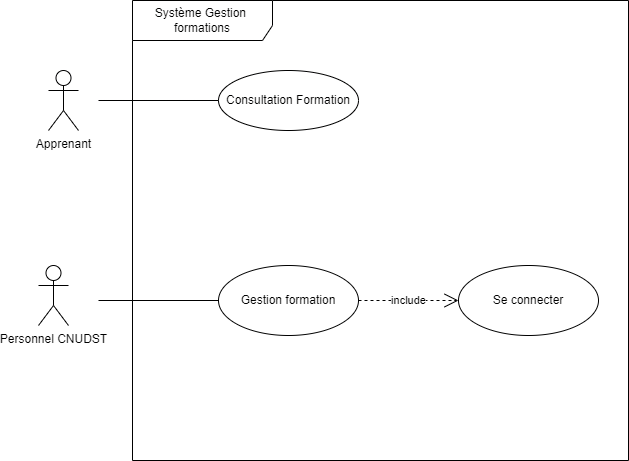
\includegraphics[width=0.75\textwidth]{D) IMAGES/globalformation.png}}
		\caption{Interface :Diagramme du cas d'utilisation global-sprint 2 }
		\label{Org}
	\end{figure}
\newpage
	\item Détails du cas d'utilisation globale<<Gestion formation>>
	
	\begin{figure}[!h]
		\centering
		{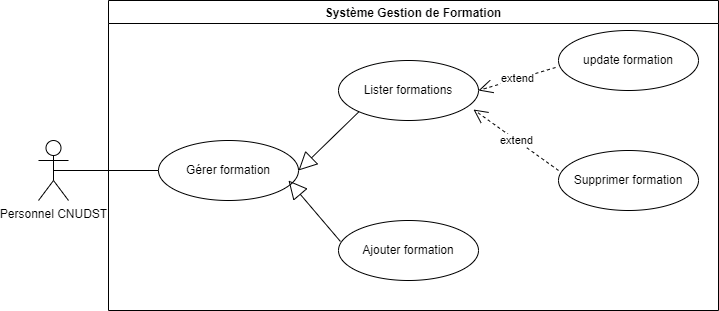
\includegraphics[width=0.95\textwidth]{D) IMAGES/Gestform.png}}
		\caption{Interface :Détails du cas d'utilisation "Gestion formation" }
		\label{Org}
	\end{figure}
\item Détails du cas d'utilisation globale "Consultation formation"

\begin{figure}[!h]
	\centering
	{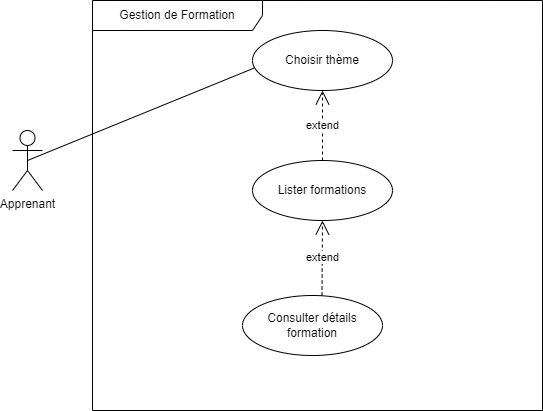
\includegraphics[width=0.75\textwidth]{D) IMAGES/detail2.png}}
	\caption{Interface :Détails du cas d'utilisation "Consultation formation" }
	\label{Org}
\end{figure}
\end{itemize}
\section{Description textuelle des cas d'utilisation}
\subsection{Cas d'utilisation "Consulter formation"}
\textbf{Description textuelle du cas d'utilisation : Consulter formation}\\
\textbf{Titre :} Cas d'utilisation: consulter formation\\
\textbf{But:} Citer les étapes permettant à un visiteur de consulter la liste et les détails des formations fournies par le CNUDST.\\
\textbf{Acteur Principal:} visiteur\\
\textbf{Date de création:} 19/07/2022\\
\textbf{Date de mise à jour:} 21/07/2022\\
\textbf{Responsable:} Olfa CHAOUECH\\
\textbf{Version:} 1.0\\
\textbf{Description des scénarii:}\\
Le cas d'utilisation commence quand un visiteur est connecté au site web et il est sur la page d'accueil.

	 \textbf{Pré condition:}\\
	Le visiteur est sur notre page d'accueil.\\
	\textbf{Scénario nominal:}
	\begin{enumerate}
		\item Le visiteur choisit un thème et clique dessus.
		\item le système affiche la liste de toutes les formations liées au thème choisi.
		\item le visiteur choisit une formation et clique dessus.
		\item le système affiche les détails de cette formation.

    \textbf{Scénario Alternatif A:}\\
    A1 : Le visiteur est sur la page de formations(Programs) et veut consulter les autres formations disponibles.
    $\rightarrow$ L'enchaînement A1 démarre au point 4 du scénario nominal.
    \item Le visiteur clique sur le thème et revient à la liste des formations.
    $\rightarrow$ Le scénario reprend au point 2.
    
\textbf{Scénario d'exception E:}\\
E1 : Le visiteur ne trouve pas la formation souhaitée.
$\rightarrow$ L'enchaînement E1 démarre au point 2 du scénario nominal.

\item Le visiteur termine sa visite en quittant la page.
\end{enumerate}
\textbf{Post-condition:}
Le visiteur a consulté les détails des formations.
\subsection{Cas d'utilisation "Ajouter formation"}
\textbf{Description textuelle du cas d'utilisation : Ajouter formation}\\
\textbf{Titre :} Cas d'utilisation: ajouter formation\\
\textbf{But:} Détailler les étapes permmettant à un administrateur d'ajouter une ou plusieurs formations.\\
\textbf{Acteur Principal:} administrateur\\
\textbf{Date de création:} 15/06/2022\\
\textbf{Date de mise à jour:} 24/06/2022\\
\textbf{Responsable:} Olfa CHAOUECH\\
\textbf{Version:} 1.0\\
\textbf{Description des scénarii:}\\
Le cas d'utilisation commence quand l'administrateur est connecté et il est sur la page de menu de Wordpress.

\textbf{Pré condition:}\\
L'administrateur est sur la page de menu de wordpress.\\
\textbf{Scénario nominal:}
\begin{enumerate}
	\item L'administrateur clique sur le type de contenu Programs.
	\item Le système affiche un menu pour ajouter une formation. 
	\item L'administrateur remplit les champs.
	\item L'administrateur clique sur le bouton ajouter.
	
	\textbf{Scénario Alternatif A:}\\
	A1 : L'administrateur est sur la page de menu et veut ajouter une autre formation.
	$\rightarrow$ L'enchaînement A1 démarre au point 3 du scénario nominal.
	
	
	\textbf{Scénarion d'exception E:}\\
	E1 : L'administrateur ne remplit pas les champs.
	$\rightarrow$ L'enchaînement E1 démarre au point 3 du scénario nominal.
	
	\item L'administrateur ajoute l'ensemble des formations et quitte la page.
\end{enumerate}
\textbf{Post-condition:}
Toutes les formations ont été ajoutées par l'administrateur.
\subsection{Cas d'utilisation "Lister formation"}
\textbf{Description textuelle du cas d'utilisation : Lister formation}\\
\textbf{Titre :} Cas d'utilisation: lister formation\\
\textbf{But:} Détailler les étapes permettant à un administrateur d'afficher la liste des formations.\\
\textbf{Acteur Principal:} administrateur\\
\textbf{Date de création:} 28/06/2022\\
\textbf{Date de mise à jour:} 01/07/2022\\
\textbf{Responsable:} Olfa CHAOUECH\\
\textbf{Version:} 1.0\\
\textbf{Description des scénarii:}\\
Le cas d'utilisation commence quand l'administrateur est connecté et il est sur la page de menu de Wordpress.

\textbf{Pré condition:}\\
L'administrateur est sur la page de menu de wordpress.\\
\textbf{Scénario nominal:}
\begin{enumerate}
	\item L'administrateur clique sur le type de contenu Programs puis sur ALL Programs .
	\item Le système récupère les données des formations de la base. 
	\item Le système affiche la liste de toutes les formations disponibles et en face de chacune il existe deux options: un choix pour "Edit" et un choix pour "Delete" une formation.
	\item L'administrateur consulte la liste des formations.
	\item L'administrateur choisit une formation et choisit une option.
	\item Modification
	\begin{itemize}
		\item L'administrateur clique sur "edit";
		\item Le système affiche une interface de mise à jour d'une formation;
		\item L'administrateur modifie les champs désirés;
		\item L'administrateur clique sur update;
		\item Le système met à jour les données de la formation dans la base;
	\end{itemize}
	
	\item Suppression
	\begin{itemize}
		\item L'administrateur clique sur "delete";
		\item Le système affiche un message de confirmation;
		\item L'administrateur confirme la suppression;
	\end{itemize}
	
	\textbf{Scénario Alternatif A:}\\
	A1 : L'administrateur est sur la page de mise à jour d'une formation et veut modifier une autre.
	$\rightarrow$ L'enchaînement A1 démarre au point 3 du scénario nominal
	.
	
	
	\textbf{Scénario d'exception E:}\\
	E1 : L'administrateur change d'avis et veut abandonner la consultation des formations et les opérations de modification et de suppression.
	$\rightarrow$ L'enchaînement E2 démarre au point 3 du scénario nominal.
	
	\item L'administrateur quitte la page.
\end{enumerate}
\textbf{Post-condition:}
L'administrateur effectue les modifications désirées.
\section{Conception}
\subsection{Diagramme des séquences}
\newpage
\begin{itemize}
	
	\item Diagramme de séquence "Consulter formations"
	\begin{figure}[!h]
		\centering
		{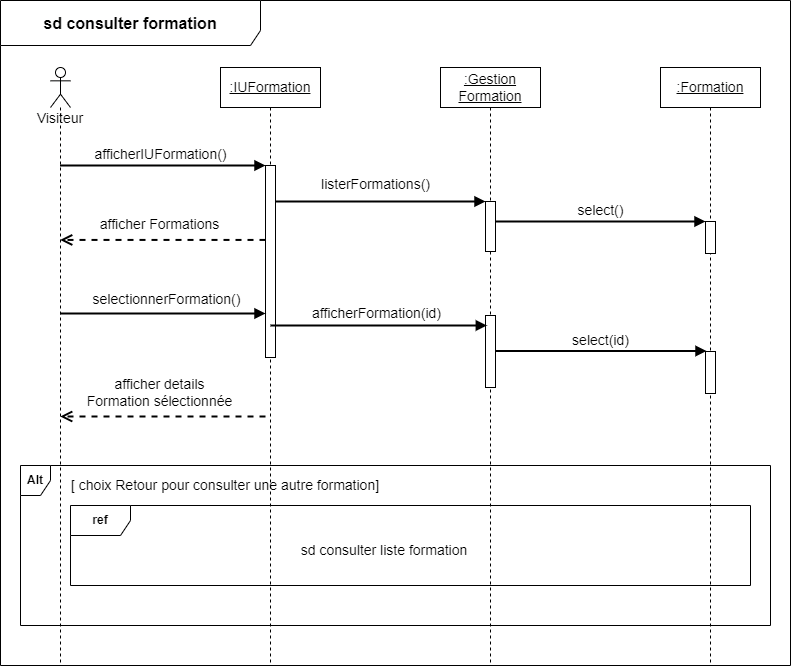
\includegraphics[width=1\textwidth]{D) IMAGES/seqconfor.png}}
		\caption{diagramme de séquence: consulter formation}
		\label{Diagramme3}
	\end{figure}

\newpage




\item Diagramme de séquence "ajouter formation"

\begin{figure}[!h]
	\centering
	{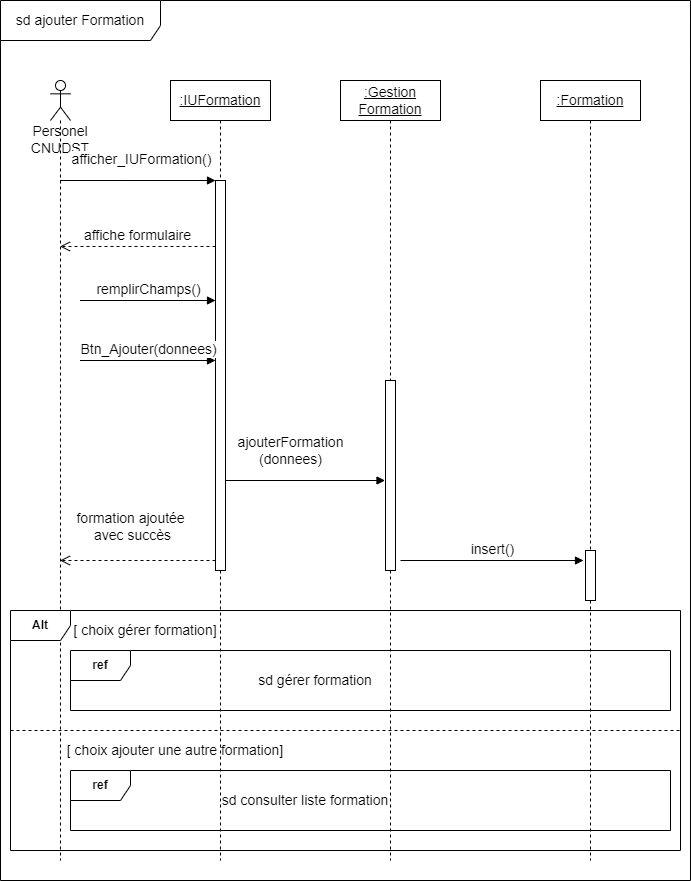
\includegraphics[width=0.95\textwidth]{D) IMAGES/seqform2.png}}
	\caption{diagramme de séquence: ajouter formation}
	\label{Diagramme3}
\end{figure}
\newpage
\item Diagramme de séquence "lister formations"
\begin{figure}[!h]
	\centering
	{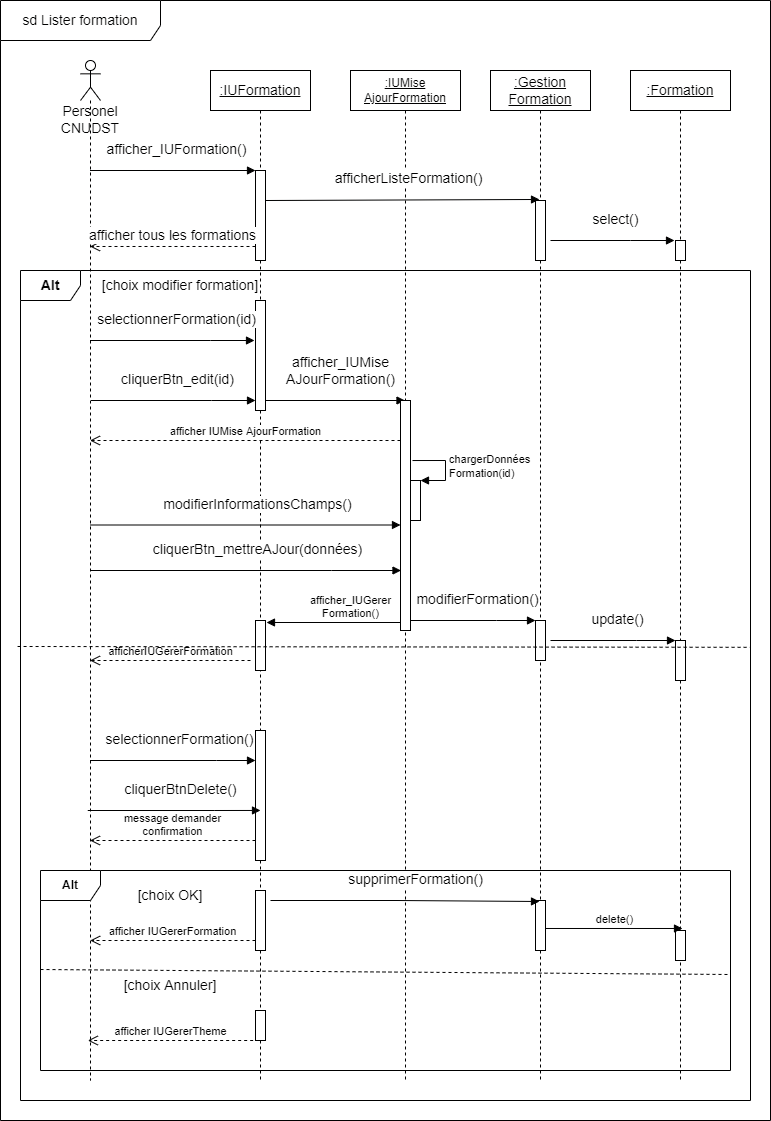
\includegraphics[width=0.75\textwidth]{D) IMAGES/seqforlist.png}}
	\caption{diagramme de séquence: lister formations}
	\label{Diagramme3}
\end{figure}
\newpage
\end{itemize}
\subsection{Diagramme de classes}
La figure ci-dessous correspond au diagramme de classes de notre site, elle représente ses classes, ses méthodes, ses associations et ses propriétés.
\begin{figure}[!h]
	\centering
	{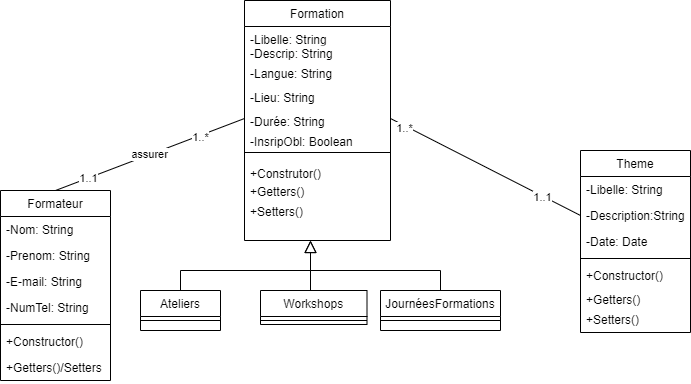
\includegraphics[width=0.75\textwidth]{D) IMAGES/diagClassFor.png}}
	\caption{diagramme de classes sprint 2}
	\label{Diagramme3}
\end{figure}
\section{Réalisation}
\subsection{Description des interfaces}
\begin{itemize}
	\item \textbf{Interface : Interface de la page d'accueil}
	\newpage
	\begin{figure}[!h]
		\centering
		{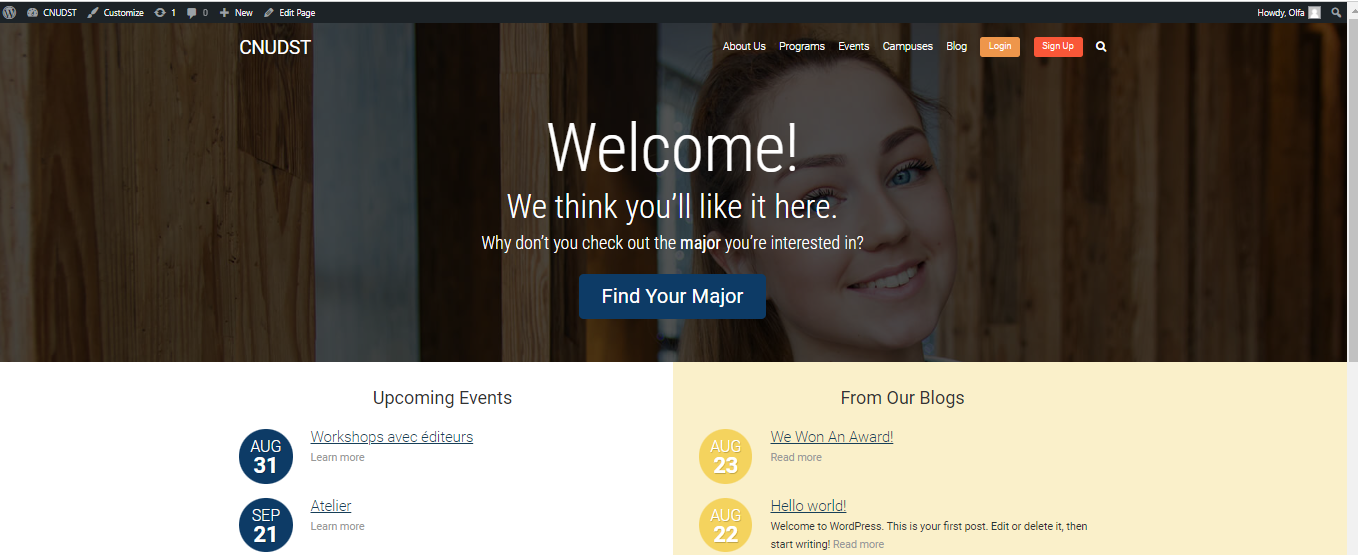
\includegraphics[width=1.05\textwidth]{D) IMAGES/them.png}}
		{
\includegraphics[width=1.05\textwidth]{D) IMAGES/them2.png}}
		\caption{Interface de la page d'accueil}
		\label{Org}
	\end{figure}
	Cette page est la première qui s'affiche quand l'utilisateur visite notre site. Elle lui permet d'avoir une idée sur les thèmes de formations futures (Upcoming Events).
	En cliquant sur le bouton "Find your Major", le visiteur peut lister les formations organisées par le CNUDST.\\
	Sur cette page le visiteur trouve une barre de menu qui lui permettra de naviguer vers les différentes pages du site.\\
	\newpage
	\textbf{Interface: Consultation de la liste des thèmes}\\
	Cette page permet au visiteur d'afficher la liste des thèmes (All Events), aussi elle contient un lien qui permet d'afficher l'ensemble des évènements passés.\\
	\begin{figure}[!h]
		\centering
		{
\includegraphics[width=1.05\textwidth]{D) IMAGES/listevent.png}}
		\caption{Interface : Consultation de la liste des thèmes }
		\label{Org}
	\end{figure}\\
	\textbf{Interface: Consultation de la liste des formations}\\
	Cette page permet d'afficher la liste des formations qui vont être organisées par le CNUDST.
	\begin{figure}[!h]
		\centering
		{
\includegraphics[width=1.05\textwidth]{D) IMAGES/allprog.png}}
		\caption{Interface : Consultation de la liste des formations }
		\label{Org}
	\end{figure}\\
\newpage
	\textbf{Interface : Détails formations}\\
	\begin{figure}[!h]
		\centering
		{
\includegraphics[width=1.05\textwidth]{D) IMAGES/detfor.png}}
		{\includegraphics[width=1.05\textwidth]{D) IMAGES/detfor2.png}}
		{\includegraphics[width=1.05\textwidth]{D) IMAGES/detfor3.png}}
		\caption{Interface : détails formations}
		\label{Org}
	\end{figure}
	Cette page permet au visiteur de consulter les détails d'une formation. \\
	\textbf{Interface : Gérer les formations par l'administrateur (lister, ajouter, modifier et supprimer)}\\
	C'est une interface qui permet à l'administrateur d'ajouter, lister, modifier et supprimer une formation.
	\newpage 
	\begin{figure}[!h]
		\centering
		{\includegraphics[width=1.05\textwidth]{D) IMAGES/Gerer.png}}
		\caption{Interface : Gérer les formations par l'administrateur }
		\label{Org}
	\end{figure}
\end{itemize}
\textbf{Conclusion}\\
Dans ce chapitre, nous avons essayé de mettre le focus sur le développement du deuxième sprint qui a duré quatre semaines.\\
Dans ce qui suit, nous allons entamer le dernier sprint de notre processus de développement des EPIC: \begin{itemize}
	\item Inscription à une formation en lige
	\item Interaction sur le site
\end{itemize}.






\chapter{Sprint 3: Inscription et interaction à une formation en ligne}%
\label{chap:5}
\input{Chapitre5.tex}
\chapter*{Conclusion Générale}
\label{chap:Conclusion Générale}
\markboth{\MakeUppercase{Conclusion Générale}}{}%
\addcontentsline{toc}{chapter}{Conclusion Générale}
Ce travail est l'aboutissement de trois années de formation en technologie de l'informatique, spécialité DSI à ISET Rades.\\
Cette formation s'est achevée par un stage de fin d'études (PFE) effectué au sein du CNUDST durant la période qui s'est étalée entre 11/04/2022 et 09/09/2022. Au terme duquel, nous avons été amenés à concevoir et implémenter un thème et un plugin Wordpress afin de permettre à la société d'accueil de gérer les formations en ligne qu'elle organise périodiquement au profit de la communauté scientifique tunisienne.\\
Pour atteindre cet objectif, nous avons commencé par analyser le contexte général du projet en effectuant une analyse afin de comprendre les différentes exigences demandées.\\
Par la suite, nous avons préparé un planning de travail selon l'approche SCRUM.\\ Cette phase fondamentale nous a permis de fixer les objectifs de notre release qui est composée de trois sprints.\\
Tout au long de cette phase, nous avons pu fixer les acteurs principaux, nous avons spécifié les différents besoins fonctionnels et non fonctionnels, par la suite nous avons construit le backlog du produit pour que nous puissions piloter le projet par l'approche SCRUM.\\
Ce travail nous a été très instructif de point de vue des connaissances acquises. Il nous a donné l'opportunité pour confirmer une fois de plus nos connaissances dans le développement PHP.\\
De plus, ce projet nous a donné l'occasion d'étudier et d'utiliser le CMS Wordpress pour développer des plugins.\\
Certes, comme tout système, cette application n'est pas "exemptus" de limites. Certaines fonctionnalités pourraient être améliorées et donner lieu à plusieurs autres extensions.
Comme perspective, nous proposons à l'entreprise d'accueil "CNUDST" d'utiliser un framework tel que Laravel au lieu de Wordpress, car ce dernier ne permet pas de répondre à toutes les spécificités demandées.\\
Aussi nous recommandons vivement l'ajout d'un tableau de bord afin d'assurer la visualisation des données et d'évaluer la situation de l'entreprise d'une manière globale par département, région ou même par équipes.
 % Ce rapport avait pour objet de décrire les fonctionnements et le rôle du Centre National Universitaire de Documentation Sceintifique et Technique, lieu où j’ai effectué mon stage de perfectionnement.\\
  %Pendant la période passée au sein de cette entreprise, j’ai eu l’opportunité de mettre en pratique mes
  %connaissances théoriques et techniques acquises au long de ma formation à ISET Rades.\\
  %Ce stage représente pour moi une bonne experience dans le monde de développement et de création de
  %projets.

\newpage
\appendix
\addcontentsline{toc}{chapter}{Annexes}
\markboth{\MakeUppercase{Annexe}}{}

\chapter{Mind Map du projet créé avec Coggle}
\label{chap:appendix}



\begin{figure}[!h]
	\centering
	{\includegraphics[width=0.95\textwidth]{D) IMAGES/map.png}}
	\caption{Diagramme du Projet}
	\label{Org}
\end{figure}
%\section{Code R pour les modèles}

 %An appedix if you need it.
 
 %\begin{verbatim}
%Insérer ici le code !
% \end{verbatim}

%\section{Librairies utilisées}
 
 % Lorem ipsum dolor sit amet, consectetur adipisicing elit, sed do eiusmod
 %tempor incididunt ut labore et dolore magna aliqua. Ut enim ad minim veniam,
 % quis nostrud exercitation ullamco laboris nisi ut aliquip ex ea commodo.


%%%%%%%%%%%%%%%%%%%%%%%%%%%%%%%%%%%%%%%%%%%%%%%%%%%%
% Don't touch this, it is auto generated
%%%%%%%%%%%%%%%%%%%%%%%%%%%%%%%%%%%%%%%%%%%%%%%%%%%%
\nocite{*}

%\phantomsection{}
%\addcontentsline{toc}{chapter}{Webography}
%\printbibliography[title={Webography},type=online]

%\phantomsection{}
%\addcontentsline{toc}{chapter}{Bibliography}
%\printbibliography[title={Bibliography},nottype=online]

%\printbibheading %exemple de bibliographie divisée en sections. Pour ajouter des oeuvres non citées,utiliser \nocite

%\printbibliography[keyword=pratique,heading=subbibliography,title={Théories littéraires dans les jeux vidéo}]
%\printbibliography[keyword=litteraire,heading=subbibliography,title={Narratologie et structuralisme}]

%\printbibliography[keyword=jeu,heading=subbibliography,title={\emph{Games studies}}]

\bibliographystyle{apalike}
%\bibliographystyle{plain}

\bibliography{Biblio.bib}

%\cleardoublepage%

\addtocontents{toc}{\protect\setcounter{tocdepth}{3}}

\printglossaries
\printindex

%\begin{abstract}

Ce travail s’inscrit dans le cadre du Projet de Fin d'Etudes réalisé au sein de \studyDepartment.\\ 
L’objectif de ce projet consiste à automatiser la gestion des formations organisées par Le Centre National Universitaire de documentation Scientifique et Technique (CNUDST) périodiquement au profit de la communauté scientifique tunisienne. 

% les tests de performance 
\keywords{}
\keywordss{SCRUM, PHP, MySql, Wordpress, Agil, UML} \\

\vspace{1.5cm}
\centerline{\bf Abstract}
\vspace{0.6cm}

The present work is part of a graduation project carried out within the company \studyDepartment.\\ This project aims to automate the management of formation organized by the National University Center for Scientific and Technical Documentation (CNUDST) periodically for the benefit of the Tunisian scientific community.\\

\keywords{}
\keywordss{SCRUM, PHP, MySql, Wordpress, Agil, UML}
\end{abstract}



\end{document}
